\chapter{基于机器学习预测龙子祠泉流量}\label{chap:ml_spring}

第\ref{chap:ml_sunspot}章基于一种特征(太阳黑子强度)研究时间序列数据。在本章的研究中,输入数据的特征(历史泉流量和降雨量)有所增加,利用机器学习探索龙子祠泉流量动态变化趋势。因此,本章可以检验增加特征种类对机器学习探索时间序列数据的影响。

\section{研究背景}\label{sec:spr_background}

近几十年来,全球人口持续增长,生活用水和农业用水的需求也随之增长,淡水短缺现象日益严重\citep{portmann2010mirca2000,iglesias2015adaptation}。地下含水层中存储着大量的未冻结淡水,这些淡水有助于人类生存的可持续发展。然而,全球地下水每年消耗\sim\SI{283}{km^{3}/year},出现了一定程度的过度开采\citep{wada2010global}。地下水过度开采的后果包括井水干涸、溪流和湖泊水量减少、水质退化、抽水成本增加、地面沉降、油井产量下降等\citep{bartolino2003ground,nayak2006groundwater}。\citet{dalin2017groundwater}和\citet{butler2018sustainability}研究表明,灌溉是地下水损耗的主要原因。

有效管理水资源是一项艰巨的任务,需要考虑到不同的时间尺度\citep{galelli2010building}。\citet{kresic2009groundwater}在水资源管理中引入了可持续发展的概念,对泉流量进行了深入研究。\citet{coppola2003artificial}指出,地下水位预测对于实施最佳水管理政策和跨地缘政治保护水资源政策至关重要。地下水是一种可再生资源,在干旱时期地下水具备良好的抵御能力。通常地下水资源按半季节至季节进行规划,优化水的利用效率,可保持农地的土壤含水容量以及维持水系统平衡。

过去的几十年里,由数据驱动的模型在水文领域的应用发展迅速,综述见\citep{abrahart2012two,deka2014support}。应用领域包括降水---径流模型\citep{dibike2001model,solomatine2003model,granata2016support}、土壤湿度\citep{ahmad2010estimating}、干旱预测\citep{le2016meteorological}、废水质量指标\citep{granata2017machine}。还有一些其他的研究,例如,采用树模型或集成方法预测洪水事件\citep{solomatine2004m5}、年均洪水\citep{singh2010estimation}、波浪冲刷深度\citep{etemad2011model}、河流产沙量\citep{goyal2014modeling}、桥墩周围的最大冲刷深度\citep{najafzadeh2016prediction}、下游水闸的局部冲刷深度\citep{najafzadeh2017prediction}、废水水力学问题\citep{granata2017machine}、评估泥沙输移\citep{najafzadeh2017application}、主河道和漫滩的流量\citep{zahiri2018optimized}等。

已有研究表明,利用机器学习预测地下水水位具备可行性。例如,\citet{coppola2003artificial}利用ANNs预测地下水位;\citet{sun2013predicting}通过空间插值技术耦合数据驱动模型预测地下水水位变化;\citet{tapoglou2014spatio}基于混合ANN--Kriging模型,模拟德国巴伐利亚州Isar河流域的每日地下水水位变化;\citet{Sun2015Technical}基于ANNs预测新加坡沼泽森林地下水位变化;\citet{yadav2017assessing}比较了极端学习机和SVM在预测加拿大两个不同油井的月度地下水水位方面的性能,发现极端学习机的表现优于SVM;\citet{sahoo2017machine}使用微分机器学习算法预测高平原含水层和密苏里河流域的水位变化,利用光谱分析确定合成输入,将获得的结果输入ANNs,得出ANNs优于混合线性和非线性回归模型;\citet{guzman2017use}采用非线性自回归神经网络预测密西西比河含水层中井水水位;\citet{wunsch2018forecasting}也使用非线性自回归神经网络对德国西南部的几个油井预测每月地下水水位,表明了非线性自回归神经网络预测地下水水位具备优势;\citet{amaranto2018semi}比较了五种不同的数据驱动模型在不同水文状况下季节性地下水水位的预测性能,发现所有由数据驱动的模型均优于基线模型,且在缺水条件下误差有所增加;\citet{Rakhshandehroo2018Long}基于小波神经网络预测佛罗里达州浅井和阿肯色州深井的地下水水位,得出浅井中嘈杂的地下水波动导致误差更高;\citet{amaranto2019spatially}利用两步数据驱动建模方法,基于气候变量、地表水可用量、地下水位变化和人类水管理预测未来地下水可用量。

泉流量在地下水研究中非常重要\citep{toth1971groundwater,toth1999groundwater}。泉流量代表了地下水到地表水的过渡指标,反映了含水层的动态变化以及整个水流系统的运转情况。泉流量是一系列动态变化的结果,主要受该地区降水量的影响。此外,泉流量本身还会影响着泉域排入和排出的水量。水平衡条件表明,补给含水层中储存水的变化率与水流入和流出的速度基本平衡。一般来说,对水平衡条件进行定量分析通常需要考虑以下条件:历史泉流量、降水量、地下水开采量、入渗、地表径流、蒸散、地下水补给、土壤水分、侧向水流至蓄水层、地表含水层和地下含水层之间的渗漏、蓄水层中蓄水量的变化等。多数情况下,水平衡条件的评估非常复杂。

基于水平衡条件的模型来模拟泉流量的动态变化,这很难实用化。出于实际应用,研究者们经常采用更简化的方法。例如,\citet{zhang1996simulation}使用块状参数模型和最小二乘法模拟爱荷华州石灰岩含水层泉流量随时间的变化;\citet{lambrakis2000nonlinear}将非线性时间序列分析和ANNs应用于岩溶泉流量的动态变化和短期预测;\citet{hu2008simulation}基于ANNs模拟中国娘子关泉流量;\citet{fiorillo2010relation}基于互相关分析,研究了意大利南部两处岩溶泉的降水量和泉流量之间的关系;\citet{fan2013assembled}提出了组合极值统计模型,用于研究极端气候变化和高度地下水开发条件下的泉流量消耗过程;\citet{diodato2014predicting}提出了用于泉流量估算集总气候模型;\citet{cheng2021machine}利用LSTM-RNN和SVR预测了龙子祠泉未来1个月的泉流量。

本章结构安排如下。第\ref{sec:spr_data_method}节描述了数据与方法。第\ref{sec:spr_result}节描述了试验过程,并将试验结果可视化。第\ref{sec:spr_conclusion}节对试验结果进行了总结,并对下一步研究进行了展望。

\section{数据与方法}\label{sec:spr_data_method}

本节首先介绍研究区域龙子祠泉的地理条件。接着可视化分析该泉域的降水量和泉流量,找出数据的基本特征。在数据正式被训练之前,需要将原始数据集进行预处理,包括生成监督学习数据集、数据集划分、归一化处理等。最后选取几种不同的机器学习方法训练处理后的数据。

\subsection{研究区域}\label{sec:spr_area}

\begin{figure}[!htbp]
  \centering
  \includegraphics[width=0.80\textwidth]{Img/chap4_spr/spr_longzici.eps}
  \bicaption[龙子祠泉地理条件]{龙子祠泉地理条件\citep{cheng2021machine}。}{The hydrogeological conditions in Longzici Karst area \citep{cheng2021machine}.}
  \label{fig:spri_longzici}
\end{figure}

龙子祠泉域坐落于山西省临汾市,属于汾河水系。从地图上看,经度范围为$[110^\circ 45^\prime,111^\circ 30^\prime]$,纬度范围为$[35^\circ 40^\prime,36^\circ 40^\prime]$,流域面积为\sim\SI{2250}{km^{2}}。图\ref{fig:spri_longzici}绘制了龙子祠泉的地理条件。该泉域位于构造剥蚀、溶蚀中低山区,属于非全排型泉域。泉水出露于西山与临汾盆地交界处的坡积物中,可划分为东池、南池和北池3个泉。泉群露出面积为\sim\SI{0.12}{km^{2}},泉水大多以散流的形式溢出地表。

\subsection{数据描述}\label{sec:spr_deal_data}

\begin{figure}[!htbp]
  \centering
  \begin{subfigure}[b]{1.0\textwidth}
    \caption{月观测数据} 
    \vspace{-0.35cm}
    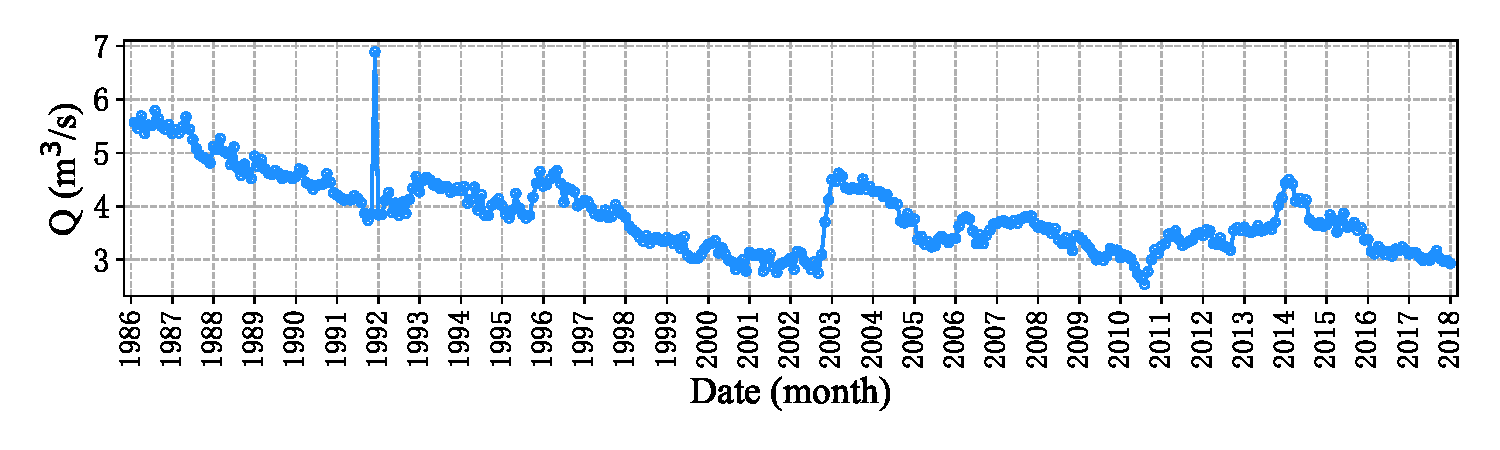
\includegraphics[width=\textwidth]{Img/chap4_spr/spr_discharge_monthly}
    \label{fig:spr_discharge_monthly}
  \end{subfigure}    \\
  \vspace{-1cm}
  \begin{subfigure}[b]{1.0\textwidth}
    \caption{年平均变化数据}
    \vspace{-0.35cm}
    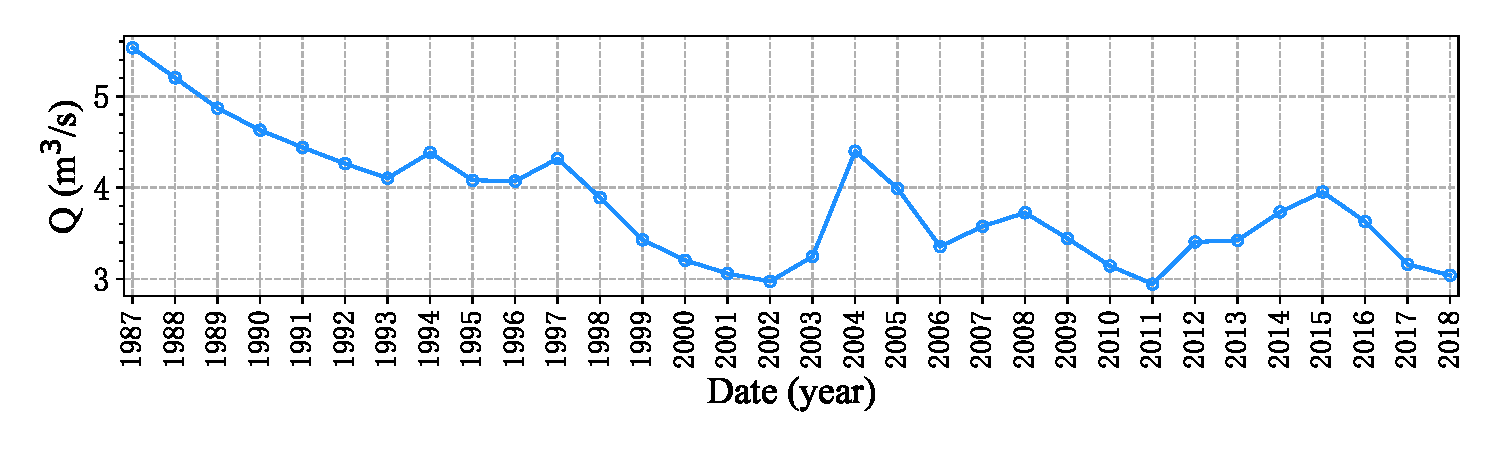
\includegraphics[width=\textwidth]{Img/chap4_spr/spr_discharge_yearly}
    \label{fig:spr_discharge_yearly}
  \end{subfigure}
  \vspace{-2cm}
  \bicaption[龙子祠泉流量变化趋势]{龙子祠泉流量变化趋势。}{The discharge variation trend of Longzici spring.}
  \label{fig:spr_discharge}
\end{figure}

针对龙子祠泉域,本研究收集了1987年1月至2018年12月(共32年)的泉流量月观测资料和泉域内化乐、克城、山头、一平垣、台头、光华、河底、双风渰、关王庙九个气象观测站的月降水资料。图\ref{fig:spr_discharge}绘制了从1987年至2018年泉流量的长时间序列。由图\ref{fig:spr_discharge_monthly}看出,这32年期间1987年7月观测到泉流量最大值\SI{5.79}{m^{3}/s}(排除了1992年11月出现的异常值),2011年7月观测到泉流量最小值\SI{2.54}{m^{3}/s}。除了突发性的泉流量增加事件外,1987年至2005年期间泉流量呈下降趋势,而2006年以后泉流量趋于稳定。出现这种现象的原因是,泉流量主要由降水量和开采量共同决定。但该地区泉水开采量数据难以收集,很难详细分析开采量对泉流量的影响。根据粗略统计的勘探数据,2003年前该地区泉水开采量保持在较高的水平(\sim 3.16$\times 10^{6}$\SI{}{m^{3}/year}),这很可能是泉流量持续下降的原因。2003年该地区出现了极端降水天气,使泉流量显著增加。在随后的几年里,泉流量波动相对规律,且略有下降趋势。由于开采量数据难以收集,本研究只关注降水量对泉流量的影响。

图\ref{fig:spr_discharge_yearly}描述了1987年至2018年年均泉流量变化趋势图。这32年来,1987年年均泉流量的观测值最大(\SI{5.53}{m^{3}/s}),2011年年均泉流量的观测值最小(\SI{2.95}{m^{3}/s})。年均泉流量的谷值分别出现在1993年、2002年、2011年,间隔为\sim 10年、这种波动可能与自然环境有关(如泉水的自我调节功能)。

\begin{figure}[!htbp]
  \vspace{-0.35cm}
  \centering
  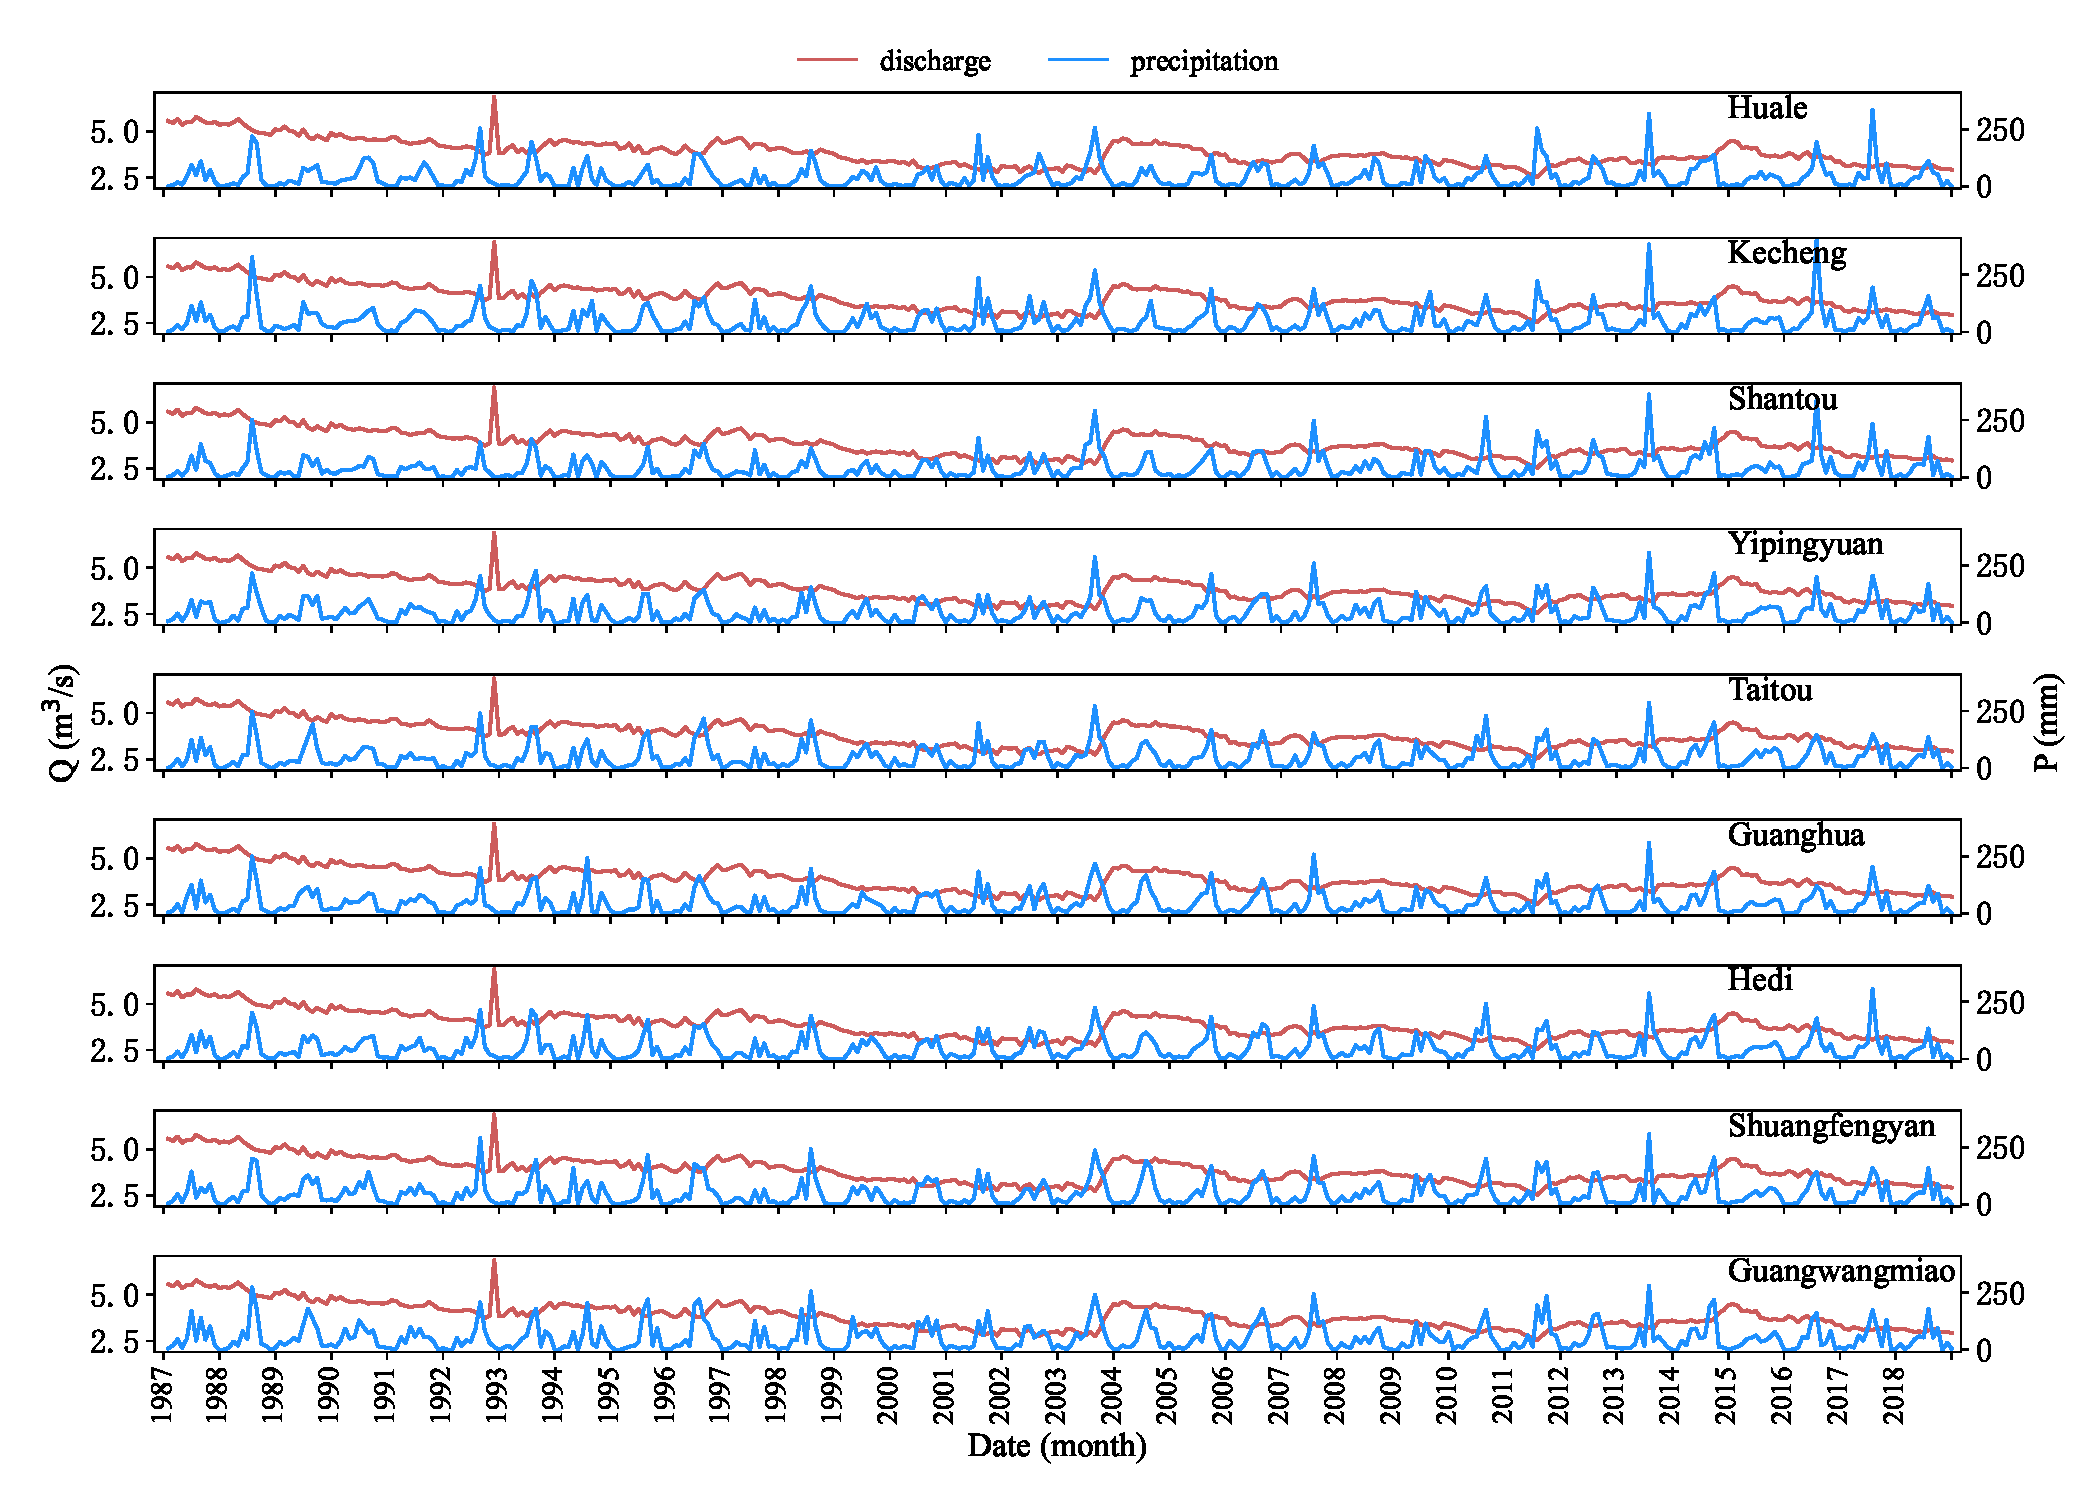
\includegraphics[width=\textwidth]{Img/chap4_spr/spr_precipitation_monthly}
  \vspace{-1cm}
  \bicaption[龙子祠泉周围9个区域降水量随时间变化的趋势图]{龙子祠泉周围9个区域(即化乐、克城、山头、一平垣、台头、光华、河底、双风渰、关王庙)降水量随时间变化的趋势图。}{The precipitation variation trend of the nine city (i.e., Huale, Kecheng, Shantou, Yipingyuan, Taitou, Guanghua, Hedi, Shuangfengyan and Guangwangmiao) around Longzici spring.}
  \label{fig:spr_precipitation_monthly}
\end{figure}

图\ref{fig:spr_precipitation_monthly}描述了1987年1月至2018年12月期间龙子祠泉周围九个区域月均降水量随时间变化的趋势图。由图\ref{fig:spr_precipitation_monthly}可知,泉域降水量在空间上的分布存在一致性波动的原则,即九个地区的降水时间序列显示出降水波动规律较为同步。另外,每年降水量也有一定的规律,夏季降水量明显上升,而冬季降水量明显下降,春季和秋季的降水量则相对平稳。

\begin{figure}[!htbp]
  \centering
  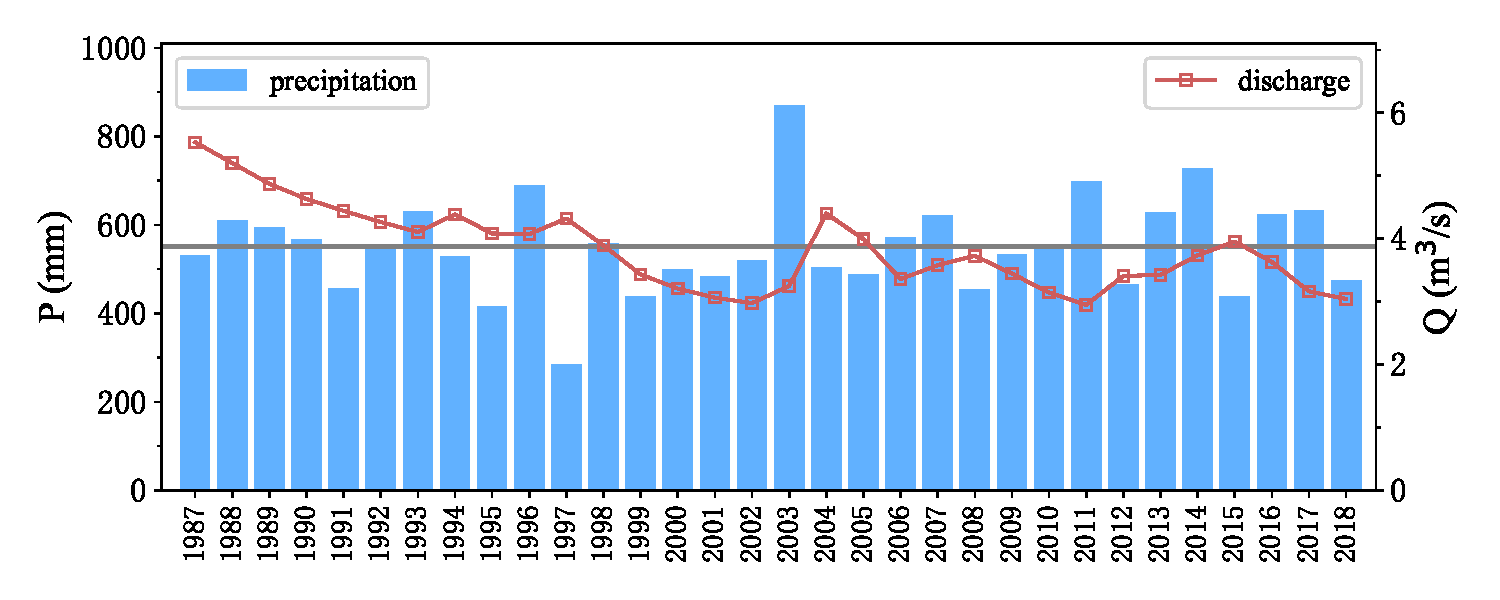
\includegraphics[width=\textwidth]{Img/chap4_spr/spr_total_precipitation_yearly}
  \vspace{-1cm}
  \bicaption[1987年至2018年期间龙子祠泉年域降水量]{1987年至2018年期间龙子祠泉年域降水量。}{The annual precipitation distribution for the area surrounding Longzici spring from 1987 to 2018.}
  \label{fig:spr_total_precipitation_yearly}
\end{figure}

\begin{figure}[!htbp]
  \centering
  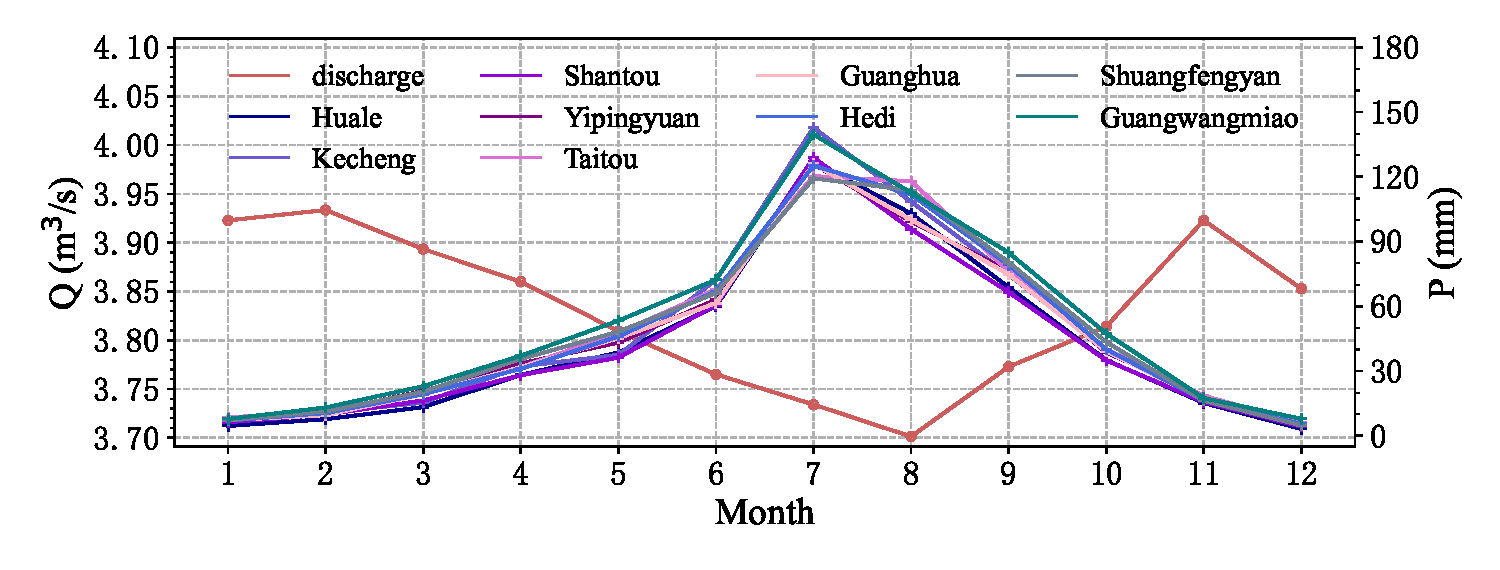
\includegraphics[width=\textwidth]{Img/chap4_spr/spr_discharge_month}
  \vspace{-1cm}
  \bicaption[龙子祠泉多年月均泉流量与降水量变化趋势]{龙子祠泉多年月均泉流量与降水量变化趋势。}{Monthly mean discharge and precipitation distribution for Longzici spring and its surrounding area.}
  \label{fig:spr_discharge_month}
\end{figure}

图\ref{fig:spr_total_precipitation_yearly}描述了泉域年际降水量分布。1987年至2018年期间,降水量变化范围为[\SI{283.79}{mm},\SI{870.60}{mm}],年均降水量为\SI{550.97}{mm}。若以年均降水量为丰枯标准,则枯水年(小于\SI{550.97}{mm})与丰水年(大于\SI{550.97}{mm})各占一半。003年年降水量为\SI{870.60}{mm},远超出其他年份,结合泉流量波动情况,得知强降水给泉流量带来了重要的水源供给,这也是泉流量在2004年迅速回升的重要原因。图\ref{fig:spr_discharge_month}中绘制了泉域九个地区多年月均泉流量与降水量的关系。由图\ref{fig:spr_discharge_month}可知,降水量是泉流量变化的重要影响因素,会直接给龙子祠泉补充水源,而且降水量对泉流量的补给响应存在$\sim$4个月的滞后。

\subsection{方法描述}\label{sec:spr_method}

本节围绕预处理方法和机器学习方法展开。未来泉流量走势主要依赖于历史泉流量和降水量,这里需要将数据集转化为监督学习时间序列数据。图\ref{fig:spr_discharge_month}表明龙子祠泉流量与降水量之间存在时间上的滞后。未来泉流量不仅依赖于历史1个月的泉流量和降水量,还可能依赖历史几个月甚至几年的泉流量和降水量。泉流量的变化趋势可被近似表达为:
\begin{equation}\adddotsbeforeeqnnum
  \label{eq:spr_sprint_precipitation}
  \begin{split}
    Q(t+\Delta,t+2\Delta,\ldots,t+f\Delta)
    =F[P_1(t),P_1(t-\Delta),\ldots,P_1(t-(n-1)\Delta);\ldots;\\
    P_9(t),P_9(t-\Delta),\ldots,P_9(t-(n-1)\Delta);\\
    Q(t),Q(t-\Delta),\ldots,Q(t-(m-1)\Delta)].
  \end{split}
\end{equation}
其中,$\Delta$代表采样间隔(1个月)。$m=n$,即假设输入的历史降水量和泉流量时间同步。$Q(t+\Delta,t+2\Delta,\ldots,t+f\Delta)$代表未来$f$个月的泉流量。$P_e(t-i\Delta)(i\in\{0,1,\ldots,n-1\},e\in\{1,2,\ldots,9\})$代表第$e$区域历史第$i$个月的降水量,$Q(t-j\Delta)(j\in\{0,1,\ldots,m-1\})$代表历史第$j$个月的泉流量。式\ref{eq:spr_sprint_precipitation}表明,输入是泉域内历史降水量与泉流量,输出为未来泉流量。

这里可用泉流量的记录有限,但这并不影响研究过程,因为本研究的目标是利用近几十年的观测数据评估模型的预测能力。小样本情况下,可以适当简化机器学习模型。龙子祠泉地理条件复杂,泉流量与降水量时间序列均呈现出复杂的非线性特征。具备喀斯特地貌特征的龙子祠泉可被视作非线性的输入/输出系统。本章选择了几种不同的机器学习方法,包括LSTM-RNN、1DCNN、LSTM-1DCNN、SVR、LR、RF、DT、KNN。

由图\ref{fig:spr_discharge_month}可知,泉流量与降水量之间存在$\sim$4个月的滞后。因此,这里考虑输入历史的泉流量和降水量为1至4个月,从而评估不同输入时间窗口对模型的影响。每个输入响应可以表示如下:
\begin{equation}\adddotsbeforeeqnnum
  \label{eq:spr_input}
  \begin{split}
    I_{-k}=[Q(t),Q(t-1),\ldots,Q(t-k+1),P_1(t),P_2(t),\ldots,P_9(t);\ldots;\\
    P_1(t-k+1),P_2(t-k+1),\ldots,P_9(t-k+1)].
  \end{split}
\end{equation}
其中,$k=1,2,3,4$。

通常地下水资源按半季节至季节进行规划,输出时间窗口可设置为1至4个月。每个输出响应可以表示如下:
\begin{equation}\adddotsbeforeeqnnum
  \label{eq:spr_output}
  O_{+f}=[Q(t+1),Q(t+2),\ldots,Q(t+f)].
\end{equation}
其中,$f=1,2,3,4$。

通过第\ref{sec:ml_slide}节的滑动窗口法,可以将原始数据集转换为监督学习数据集。紧接着,将数据集分割为训练集和测试集,分割比例为0.8:0.2。在训练集和测试集被使用之前,需要对两者分别进行归一化处理(第\ref{sec:ml_scaler}节)。

\section{试验结果与分析}\label{sec:spr_result}

在利用机器学习之前,我们首先定义一个基准模型,过去1个月的泉流量$I_{-1}$为未来1个月的泉流量$O_{+1}$,即$O_{+1}=I_{-1}$。容易得到拟合指标MSE=\SI{0.0301}{m^{3}/s}, RMSE=\SI{0.1736}{m^{3}/s}。

这里简要介绍各种机器学习的超参数配置。所有模型的输入节点数$10k$由输入时间窗口决定,输出节点数$f$由输出时间窗口决定。针对LSTM-RNN和LSTM-1DCNN,本研究采用了三层架构,LSTM-1DCNN采用了四层。采取较少的层数是因为数据集只有几百对样本,三到四层的网络足以拟合数据集。因不同网络具有的独特性质,在设置以下超参数时会有所差异。针对LSTM-RNN,前两层含LSTM神经元,最后一层为全连接层。隐藏层的节点数设为32和16,输出层为全连接层。针对1DCNN,第一层和第二层均为一维卷积层,过滤器个数、过滤器大小、步长分别为32/16、3、1。卷积层后连接了最大池化层,池化大小为2,步长为1。最后一层为全连接层。针对LSTM-1DCNN,第一层为一维卷积层,过滤器个数、过滤器大小、步长分别为128、3、1。卷积层后连接了最大池化层,池化大小为2,步长为1。第二、三层均含有LSTM神经元,神经元个数分别为64和32。最后一层为全连接层。 

以下是本章所有神经网络通用的超参数。训练经过1000回合,网络每层均会使用ReLU激活函数。批量训练数据量设为120。Adam方法作为优化器。学习率初始值设为$10^{-3}$。同时训练次数每增加10次,学习率会减小$1-10^{-6}$倍,这样逐步减小学习率能够防止模型陷入局部极小值。所有试验均使用“早停”方案,即100次迭代后,若测试集的MSE值没有下降,则停止训练。

{\footnotesize
\begin{longtable}{clcccccccc}
  \bicaption[不同模型、输入和输出时间窗口预测泉流量的拟合指标效果]{不同模型、输入和输出时间窗口预测泉流量拟合指标效果。}{Comparative indicates of testing set by using different models, input and output windows for predicting spring discharge.} 
  \label{tab:spr_indicates} \\

  \toprule
  \multicolumn{1}{c}{}&\multicolumn{1}{l}{}&\multicolumn{2}{c}{$O_{+1}$}&\multicolumn{2}{c}{$O_{+2}$}&\multicolumn{2}{c}{$O_{+3}$}&\multicolumn{2}{c}{$O_{+4}$}\\
  \cmidrule(lr){3-4} \cmidrule(lr){5-6} \cmidrule(lr){7-8} \cmidrule(lr){9-10} \noalign{\smallskip}
  \multicolumn{1}{c}{$k$} & \multicolumn{1}{l}{模型}& \multicolumn{1}{c}{MSE} & RMSE & MSE & RMSE & MSE & RMSE & MSE & RMSE\\ 
  \midrule
  \endfirsthead 

  \bicaption[不同模型、输入和输出时间窗口预测泉流量的拟合指标效果(续)]{不同模型、输入和输出时间窗口预测泉流量的拟合指标效果(续)。}{Comparative indicates of testing set by using different models, input and output windows for predicting spring discharge (continued).} \\
  \toprule
  \multicolumn{1}{c}{}&\multicolumn{1}{l}{}&\multicolumn{2}{c}{$O_{+1}$}&\multicolumn{2}{c}{$O_{+2}$}&\multicolumn{2}{c}{$O_{+3}$}&\multicolumn{2}{c}{$O_{+4}$}\\
  \cmidrule(lr){3-4} \cmidrule(lr){5-6} \cmidrule(lr){7-8} \cmidrule(lr){9-10} \noalign{\smallskip}
  \multicolumn{1}{c}{$k$} & \multicolumn{1}{l}{模型}& \multicolumn{1}{c}{MSE} & RMSE & MSE & RMSE & MSE & RMSE & MSE & RMSE\\ 
  \midrule
  \endhead 

  \bottomrule
  \endfoot

  1 & LSTM & 0.0542 & 0.2328 & 0.0013 & 0.0365 & 0.0017 & 0.0412 & 0.0022 & 0.0466\\
    & 1DCNN & 0.0542 & 0.2328 & 0.0279 & 0.1669 &  0.0197 & 0.1404 & 0.0020 & 0.0451 \\
    & LSTM-1DCNN & \textbf{0.0009} & \textbf{0.0297} & \textbf{0.0012} & \textbf{0.0352} & \textbf{0.0015} & \textbf{0.0389} & 0.0022 & 0.0474 \\
    & SVR & 0.0010 & 0.0310 &  0.0013 & 0.0361 & 0.0016 & 0.0400 & \textbf{0.0019} & \textbf{0.0433} \\
    & LR & 0.0011 & 0.0336 & 0.0015 & 0.0390 & 0.0019 & 0.0440 & 0.0023 & 0.0476  \\
    & RF & 0.0011 & 0.0338 & 0.0030 & 0.0548 & 0.0028 & 0.0528 & 0.0028 & 0.0533 \\
    & DT & 0.0075 & 0.0868 & 0.0133 & 0.1152 & 0.0079 & 0.0892 & 0.0072 & 0.0846 \\
    & KNN & 0.0015 & 0.0389 & 0.0025 & 0.0503 & 0.0032 & 0.0568 & 0.0035 & 0.0593 \\
  \hline
  2 & LSTM & 0.0542 & 0.2328 & 0.0013 & 0.0362 & 0.0019 & 0.0434 & 0.0019 & 0.0438  \\
    & 1DCNN & \textbf{0.0008} & \textbf{0.0288} & 0.0276 & 0.1660 & 0.0019 & 0.0436 & 0.0023 & 0.0484 \\
    & LSTM-1DCNN & 0.0013 & 0.0364 & 0.0015 & 0.0391 & 0.0021 & 0.0463 & 0.0026 & 0.0510 \\
    & SVR & 0.0010 & 0.0314 & \textbf{0.0013} & \textbf{0.0360} & \textbf{0.0016} & \textbf{0.0400} & \textbf{0.0018} & \textbf{0.0424} \\
    & LR & 0.0011 & 0.0326 & 0.0016 & 0.0396 & 0.0020 & 0.0452 & 0.0024 & 0.0493 \\
    & RF & 0.0043 & 0.0658 & 0.0022 & 0.0469 & 0.0028 & 0.0525 & 0.0029 & 0.0541 \\
    & DT & 0.0138 & 0.1173 & 0.0101 & 0.1007 & 0.0101 & 0.1007 & 0.0077 & 0.0879 \\
    & KNN & 0.0039 & 0.0623 & 0.0043 & 0.0654 & 0.0048 & 0.0696 & 0.0051 & 0.0716 \\
  \hline
  3 & LSTM & 0.0015 & 0.0393 & 0.0017 & 0.0415 & \textbf{0.0015} & \textbf{0.0390} & 0.0022 & 0.0466 \\
    & 1DCNN & 0.0015 & 0.0389 & 0.0017 & 0.0415 & 0.0024 & 0.0487 & 0.0024 & 0.0487 \\
    & LSTM-1DCNN & 0.0015 & 0.0382 & 0.0020 & 0.0481 & 0.0020 & 0.0450 & 0.0031 & 0.0554 \\
    & SVR & 0.0012 & 0.0345 & 0.0015 & 0.0393 & 0.0018 & 0.0422 & \textbf{0.0020} & \textbf{0.0448} \\
    & LR & 0.0016 & 0.0402 & 0.0021 & 0.0462 & 0.0025 & 0.0504 & 0.0029 & 0.0534 \\
    & RF & \textbf{0.0010} & \textbf{0.0314} & \textbf{0.0013} & \textbf{0.0360} & 0.0017 & 0.0409 & 0.0021 & 0.0455 \\
    & DT & 0.0012 & 0.0349 & 0.0031 & 0.0556 & 0.0041 & 0.0642 & 0.0044 & 0.0666 \\
    & KNN & 0.0047 & 0.0689 & 0.0053 & 0.0731 & 0.0057 & 0.0755 & 0.0057 & 0.0756 \\
  \hline
  4 & LSTM & 0.0544 & 0.2334 & 0.0020 & 0.0451 & 0.0022 & 0.0471 & 0.0023 & 0.0475 \\
    & 1DCNN & 0.0020 & 0.0444 & 0.0023 & 0.0475 & 0.0025 & 0.0504 & 0.0035 & 0.0596 \\
    & LSTM-1DCNN & 0.0024 & 0.0492 & 0.0026 & 0.0508 & 0.0028 & 0.0533 & 0.0037 & 0.0610 \\
    & SVR & 0.0013 & 0.0365 & 0.0015 & 0.0392 & 0.0019 & 0.0437 & 0.0022 & 0.0474 \\
    & LR & 0.0024 & 0.0487 & 0.0027 & 0.0519 & 0.0031 & 0.0554 & 0.0034 & 0.0585 \\
    & RF & \textbf{0.0010} & \textbf{0.0319} & \textbf{0.0014} & \textbf{0.0368} & \textbf{0.0018} & \textbf{0.0420} & \textbf{0.0022} & \textbf{0.0468} \\
    & DT & 0.0020 & 0.0442 & 0.0022 & 0.0474 & 0.0036 & 0.0597 & 0.0070 & 0.0838 \\
    & KNN & 0.0065 & 0.0808 & 0.0068 & 0.0822 & 0.0068 & 0.0824 & 0.0070 & 0.0835 \\
%   \hline
%   5 & LSTM & 0.0545 & 0.2334 & 0.0022 & 0.0464 & 0.0023 & 0.0478 & 0.0026 & 0.0509 \\
%     & 1DCNN & 0.0015 & 0.0391 & 0.0020 & 0.0452 & 0.0025 & 0.0500 & 0.0036 & 0.0603 \\
%     & LSTM-1DCNN & 0.0023 & 0.0482 & 0.0029 & 0.0536 & 0.0028 & 0.0533 & 0.0025 & 0.0499 \\
%     & SVR & 0.0013 & 0.0367 & 0.0016 & 0.0397 & 0.0021 & 0.0454 & 0.0026 & 0.0506 \\
%     & LR & 0.0026 & 0.0509 & 0.0029 & 0.0536 & 0.0033 & 0.0578 & 0.0038 & 0.0616 \\
%     & RF & \textbf{0.0011} & \textbf{0.0325} & \textbf{0.0014} & \textbf{0.0378} & \textbf{0.0018} & \textbf{0.0428} & \textbf{0.0022} & \textbf{0.0464} \\
%     & DT & 0.0018 & 0.0426 & 0.0135 & 0.1162 & 0.0037 & 0.0612 & 0.0089 & 0.0945 \\
%     & KNN & 0.0072 & 0.0848 & 0.0072 & 0.0846 & 0.0072 & 0.0851 & 0.0073 & 0.0854 \\
%   \hline
%   6 & LSTM & 0.0545 & 0.2334 & 0.0026 & 0.0510 & 0.0027 & 0.0520 & 0.0027 & 0.0515 \\
%     & 1DCNN & 0.0022 & 0.0464 & 0.0031 & 0.0555 & 0.0031 & 0.0558 & 0.0036 & 0.0603 \\
%     & LSTM-1DCNN & 0.0024 & 0.0486 & 0.0021 & 0.0456 & 0.0031 & 0.0558 & 0.0034 & 0.0582 \\
%     & SVR & 0.0012 & 0.0344 & 0.0016 & 0.0405 &  0.0021 & 0.0456 & 0.0026 & 0.0506 \\
%     & LR & 0.0024 & 0.0492 & 0.0030 & 0.0543 & 0.0035 & 0.0595 & 0.0040 & 0.0632 \\
%     & RF & \textbf{0.0011} & \textbf{0.0328} & \textbf{0.0015} & \textbf{0.0381} & \textbf{0.0019} & \textbf{0.0438} & \textbf{0.0023} & \textbf{0.0482} \\
%     & DT & 0.0013 & 0.0364 & 0.0027 & 0.0524 & 0.0054 & 0.0734 & 0.0068 & 0.0822 \\
%     & KNN & 0.0071 & 0.0845 & 0.0070 & 0.0835 & 0.0068 & 0.0827 & 0.0069 & 0.0831 \\
  \end{longtable}
}

\subsection{预测未来1个月的泉流量}\label{sec:spr_one}

\begin{table}[!htbp]
  \centering
  \bicaption[最佳模型预测2019年1月的泉流量]{最佳模型预测2019年1月的泉流量。}{Prediction the spring discharge in January 2019.}
  \label{tab:spr_one}
  \footnotesize
  \begin{tabular}{ccccc}
    \toprule
    输入时间窗口 & 1 & 2 & 3 & 4\\
    \midrule
    2019年1月的泉流量(\SI{}{m^{3}/s})& 2.97 & \textbf{2.92} & 2.99 & 2.99 \\
    \bottomrule
  \end{tabular}
\end{table}

本节讨论输出时间窗口为1个月的情况。表\ref{tab:spr_indicates}中第三至四列展示了测试阶段使用不同模型、不同输入时间窗口预测未来1个月泉流量的拟合指标效果。表\ref{tab:spr_one}展示了不同输入时间窗口下,利用最佳模型预测未来1个月的泉流量变化趋势。当输入时间窗口为1个月时,LSTM-1DCNN拟合指标MSE=\SI{0.0009}{m^{3}/s},RMSE=\\\SI{0.0297}{m^{3}/s},预测2019年1月的泉流量为\SI{2.97}{m^{3}/s};当输入时间窗口为2个月时,1DCNN拟合指标MSE=\SI{0.0008}{m^{3}/s}, RMSE=\SI{0.0288}{m^{3}/s},预测2019年1月的泉流量为\SI{2.92}{m^{3}/s};当输入时间窗口为3个月时,RF拟合指标MSE=\SI{0.0010}{m^{3}/s},RMSE=\SI{0.0313}{m^{3}/s},预测2019年1月的泉流量为\SI{2.99}{m^{3}/s};当输入时间窗口为4个月时,RF拟合指标MSE=\SI{0.0010}{m^{3}/s},RMSE=\SI{0.0319}{m^{3}/s},预测2019年1月的泉流量为\SI{2.99}{m^{3}/s}。所有模型在预测2019年1月的泉流量时,最大差距为\SI{0.06}{m^{3}/s}。

\begin{figure}[!htbp]
  \centering
  \begin{subfigure}[b]{0.305\textwidth}
    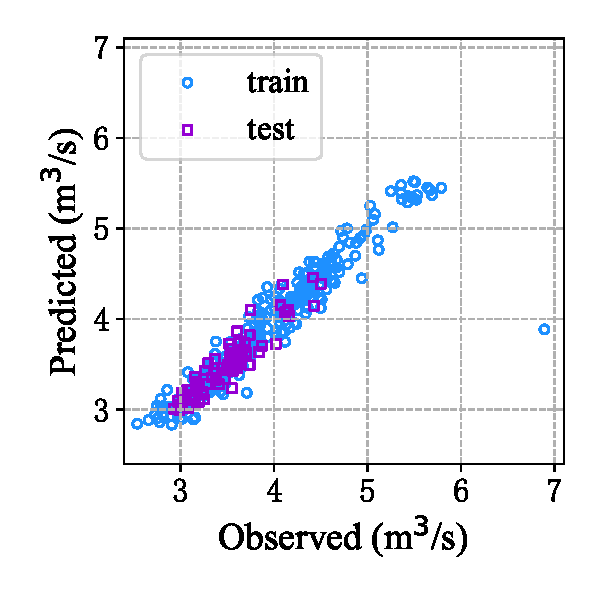
\includegraphics[width=\textwidth]{Img/chap4_spr/out1/spr_scatter_in_1_out_1_lstm_cnn.pdf}
    \vspace{-1.2cm}
    \caption{LSTM-1DCNN ($I_{-1}$)}
    \label{fig:spr_scatter_in_1_out_1_lstm_cnn}
  \end{subfigure}
  ~
  \begin{subfigure}[b]{0.615\textwidth}
    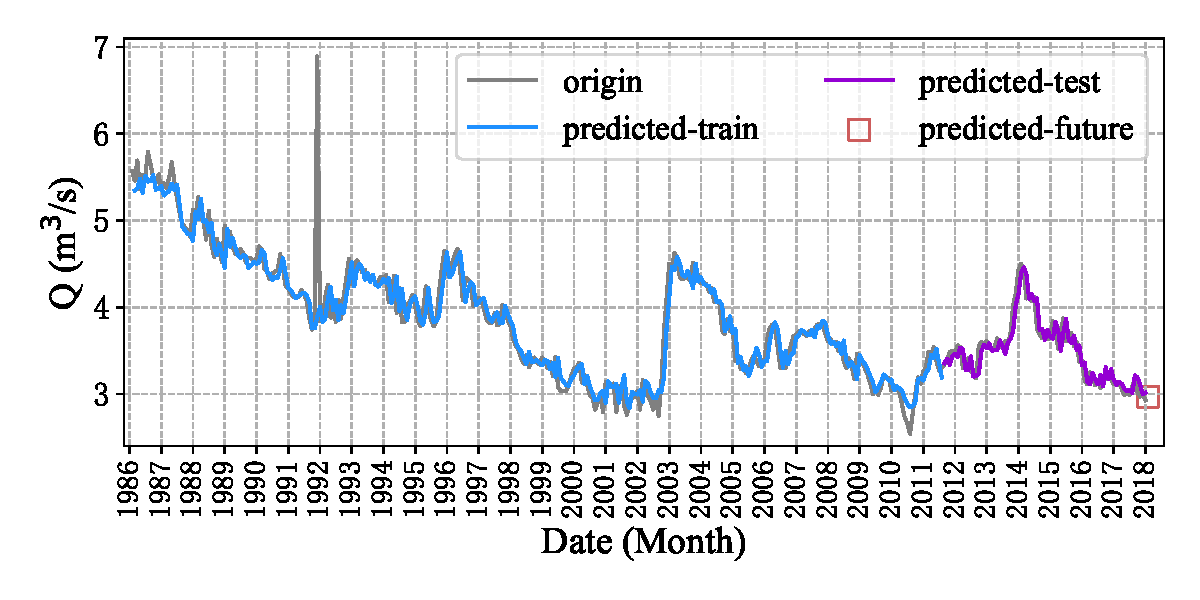
\includegraphics[width=\textwidth]{Img/chap4_spr/out1/spr_series_in_1_out_1_lstm_cnn.pdf}
    \vspace{-1.2cm}
    \caption{LSTM-1DCNN ($I_{-1}$)}
    \label{fig:spr_series_in_1_out_1_lstm_cnn}
  \end{subfigure}
  \\
  \begin{subfigure}[b]{0.305\textwidth}
    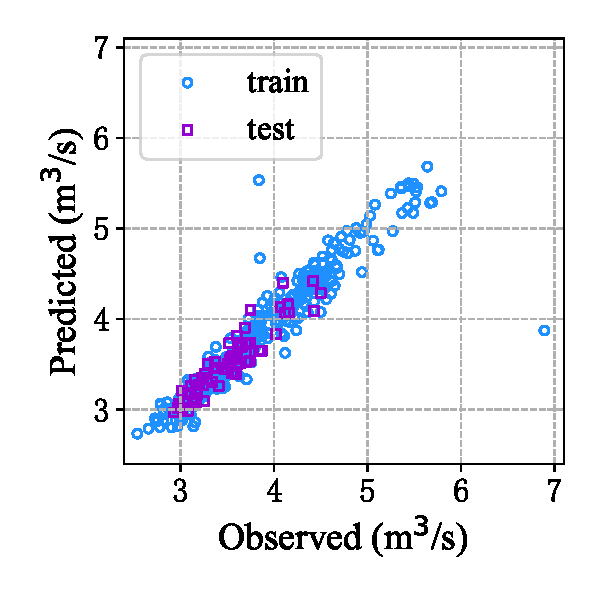
\includegraphics[width=\textwidth]{Img/chap4_spr/out1/spr_scatter_in_2_out_1_cnn.pdf}
    \vspace{-1.2cm}
    \caption{1DCNN ($I_{-2}$)}
    \label{fig:spr_scatter_in_2_out_1_cnn}
  \end{subfigure}
  ~
  \begin{subfigure}[b]{0.615\textwidth}
    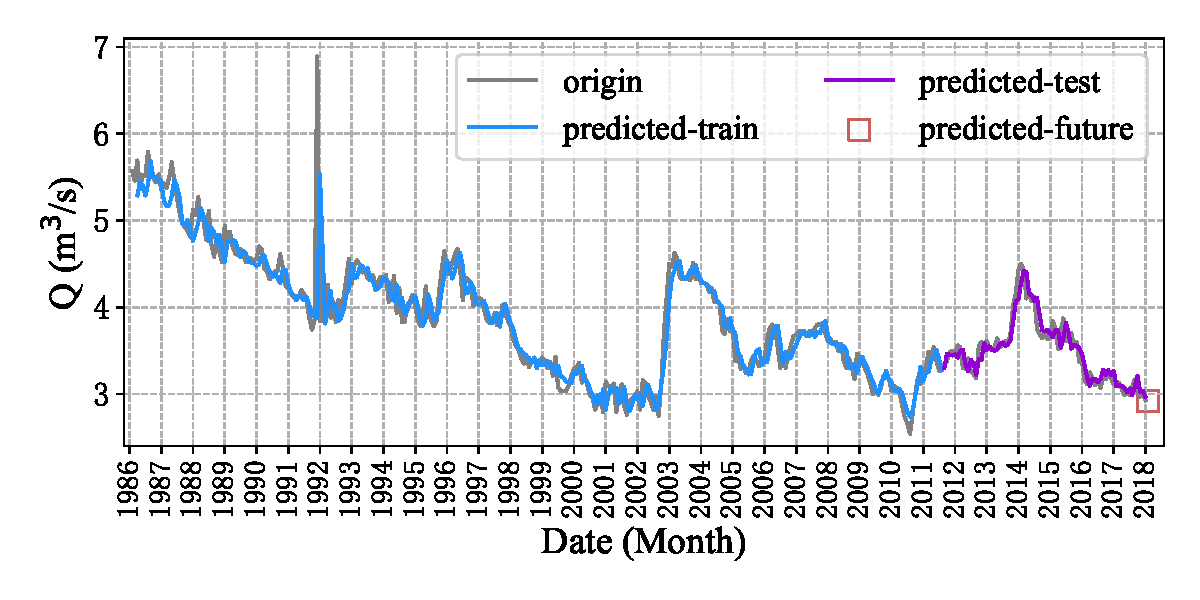
\includegraphics[width=\textwidth]{Img/chap4_spr/out1/spr_series_in_2_out_1_cnn.pdf}
    \vspace{-1.2cm}
    \caption{1DCNN ($I_{-2}$)}
    \label{fig:spr_series_in_2_out_1_cnn}
  \end{subfigure}
  \\
  \begin{subfigure}[b]{0.305\textwidth}
    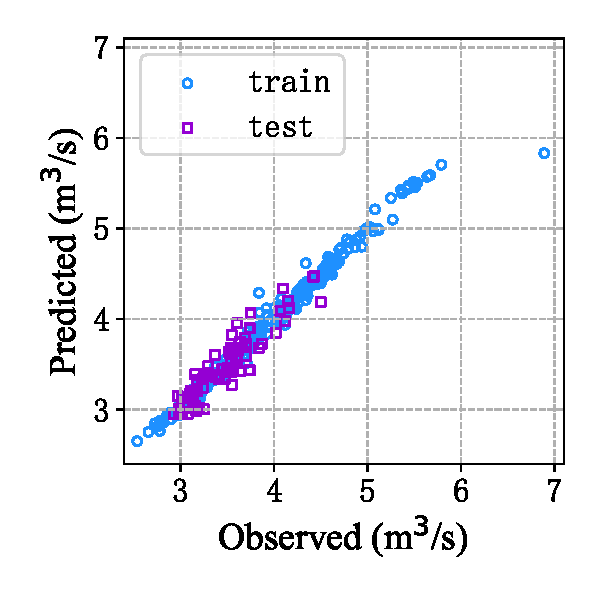
\includegraphics[width=\textwidth]{Img/chap4_spr/out1/spr_scatter_in_3_out_1_rf.pdf}
    \vspace{-1.2cm}
    \caption{RF ($I_{-3}$)}
    \label{fig:spr_scatter_in_3_out_1_rf}
  \end{subfigure}
  ~
  \begin{subfigure}[b]{0.615\textwidth}
    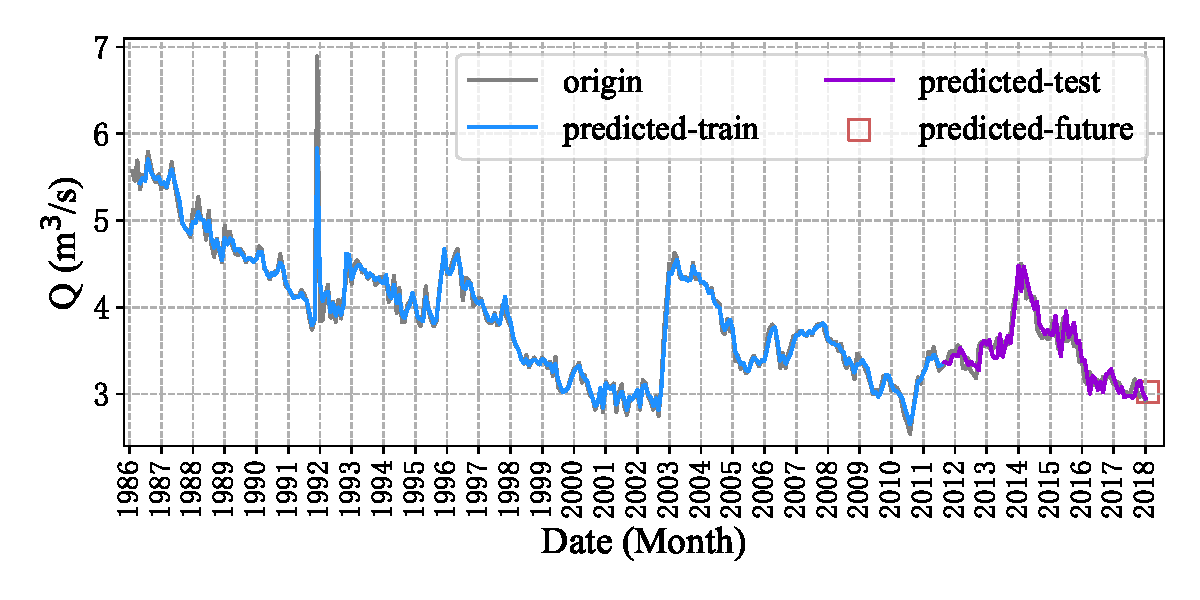
\includegraphics[width=\textwidth]{Img/chap4_spr/out1/spr_series_in_3_out_1_rf.pdf}
    \vspace{-1.2cm}
    \caption{RF ($I_{-3}$)}
    \label{fig:spr_series_in_3_out_1_rf}
  \end{subfigure}
  \\
  \begin{subfigure}[b]{0.305\textwidth}
    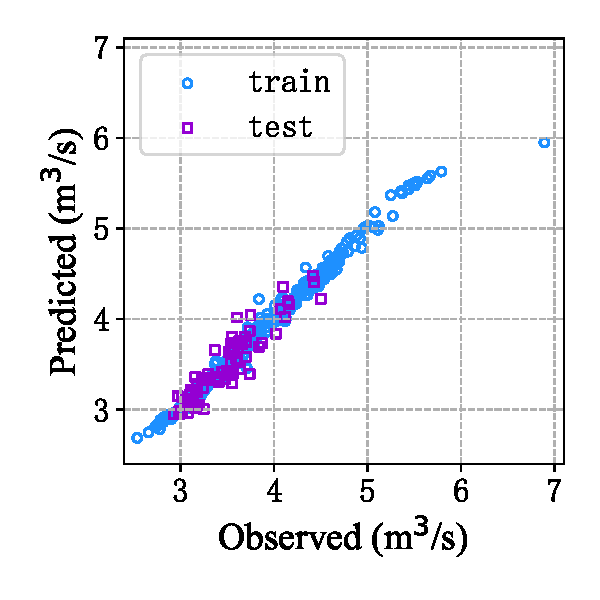
\includegraphics[width=\textwidth]{Img/chap4_spr/out1/spr_scatter_in_4_out_1_rf.pdf}
    \vspace{-1.2cm}
    \caption{RF ($I_{-4}$)}
    \label{fig:spr_scatter_in_4_out_1_rf}
  \end{subfigure}
  ~
  \begin{subfigure}[b]{0.615\textwidth}
    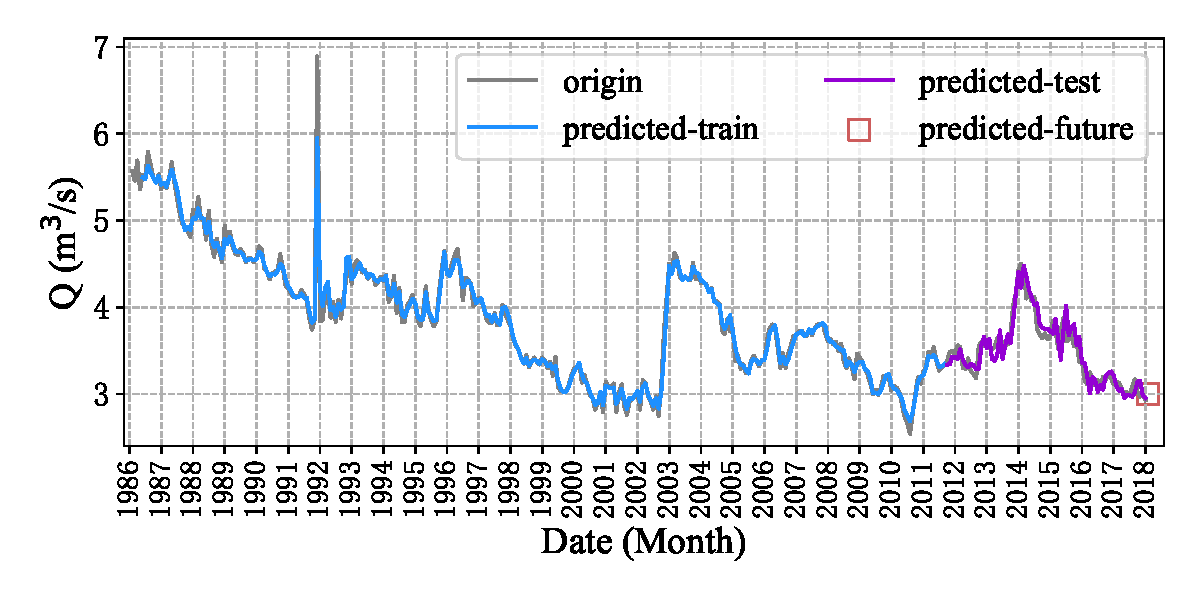
\includegraphics[width=\textwidth]{Img/chap4_spr/out1/spr_series_in_4_out_1_rf.pdf}
    \vspace{-1.2cm}
    \caption{RF ($I_{-4}$)}
    \label{fig:spr_series_in_4_out_1_rf}
  \end{subfigure}
  \bicaption[不同输入时间窗口下最佳模型预测未来1个月的泉流量]{不同输入时间窗口下最佳模型预测未来1个月的泉流量。}{Predicting the next monthly spring discharge by the best models with different input windows.}
  \label{fig:spr_out_1}
\end{figure}

图\ref{fig:spr_out_1}绘制了不同输入时间窗口下最佳模型预测未来1个月的泉流量$O_{+1}$。由图\ref{fig:spr_out_1}可知,RF均具备良好的拟合能力,且训练集中预测值和观测值时间上不存在偏差,测试集中预测值和观测值时间上存在1个月的偏差;而LSTM-1DCNN和1DCNN中的预测值和观测值在时间上存在1个月的滞后。绝大多数的预测值和观测值的绝对误差在\SI{0.1}{m^{3}/s}以内。利用这些最佳模型预测未来1个月(即2019年1月)龙子祠泉流量,均可得到较为可靠的结果。

\subsection{预测未来2个月的泉流量}\label{sec:spr_two}

\begin{table}[!htbp]
  \centering
  \bicaption[最佳模型预测2019年1月和2月的泉流量]{最佳模型预测2019年1月和2月的泉流量。}{Prediction the spring discharge in Junarary 2019 and February 2019.}
  \label{tab:spr_two}
  \footnotesize
  \begin{tabular}{ccccc}
    \toprule
    输入时间窗口 & 1 & 2 & 3 & 4\\
    \midrule
    2019年1月的泉流量(\SI{}{m^{3}/s})& \textbf{2.93} & 2.98 & 2.99 & 3.05 \\
      2019年2月的泉流量(\SI{}{m^{3}/s})& \textbf{2.94} & 2.91 & 2.93 & 3.07 \\
    \bottomrule
  \end{tabular}
\end{table}

本节讨论输出时间窗口为2个月的情况。表\ref{tab:spr_indicates}中第五、六列展示了不同模型、不同输入时间窗口下预测未来2个月泉流量的拟合指标效果。表\ref{tab:spr_two}展示了不同输入时间窗口下,利用最佳模型预测未来2个月的泉流量变化趋势。当输入时间窗口为1个月时,1DCNN拟合指标MSE=$\SI{0.0012}{m^{3}/s}$,RMSE=$\SI{0.0352}{m^{3}/s}$,预测2019年1月的泉流量为$\SI{2.93}{m^{3}/s}$,2019年2月的泉流量为$\SI{2.94}{m^{3}/s}$;当输入时间窗口为2个月时,SVR拟合指标MSE=$\SI{0.0013}{m^{3}/s}$,RMSE=$\SI{0.0360}{m^{3}/s}$,预测2019年1月的泉流量为$\SI{2.98}{m^{3}/s}$,预测2019年2月的泉流量为$\SI{2.01}{m^{3}/s}$;当输入时间窗口为3个月时,RF拟合指标MSE=$\SI{0.0013}{m^{3}/s}$,RMSE=$\SI{0.0363}{m^{3}/s}$,预测2019年1月的泉流量为$\SI{2.99}{m^{3}/s}$,2019年2月的泉流量为$\SI{2.93}{m^{3}/s}$;当输入时间窗口为4个月时,RF拟合指标MSE=$\SI{0.0014}{m^{3}/s}$,RMSE=$\SI{0.0373}{m^{3}/s}$,预测2019年1月的泉流量为$\SI{3.05}{m^{3}/s}$,预测2019年2月的泉流量为$\SI{3.07}{m^{3}/s}$。

\begin{figure}[!htbp]
\centering
  \begin{subfigure}[b]{0.305\textwidth}
    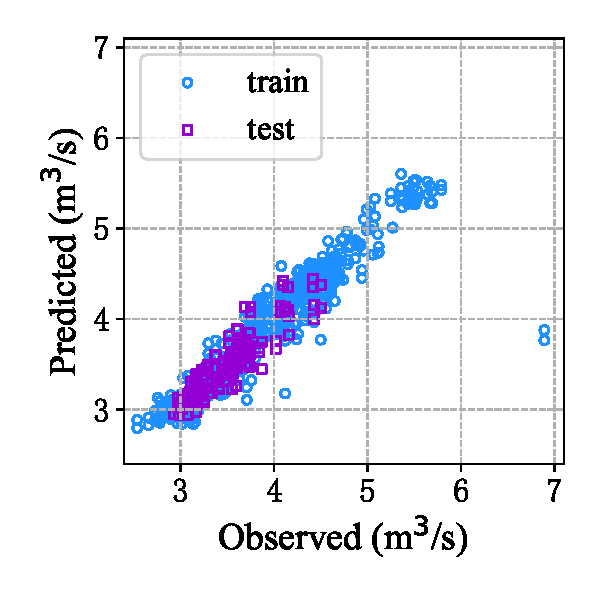
\includegraphics[width=\textwidth]{Img/chap4_spr/out2/spr_scatter_in_1_out_2_lstm_cnn.pdf}
    \vspace{-1.2cm}
    \caption{LSTM-1DCNN ($I_{-1}$)}
    \label{fig:spr_scatter_in_1_out_2_lstm_cnn}
  \end{subfigure}
  ~
  \begin{subfigure}[b]{0.615\textwidth}
    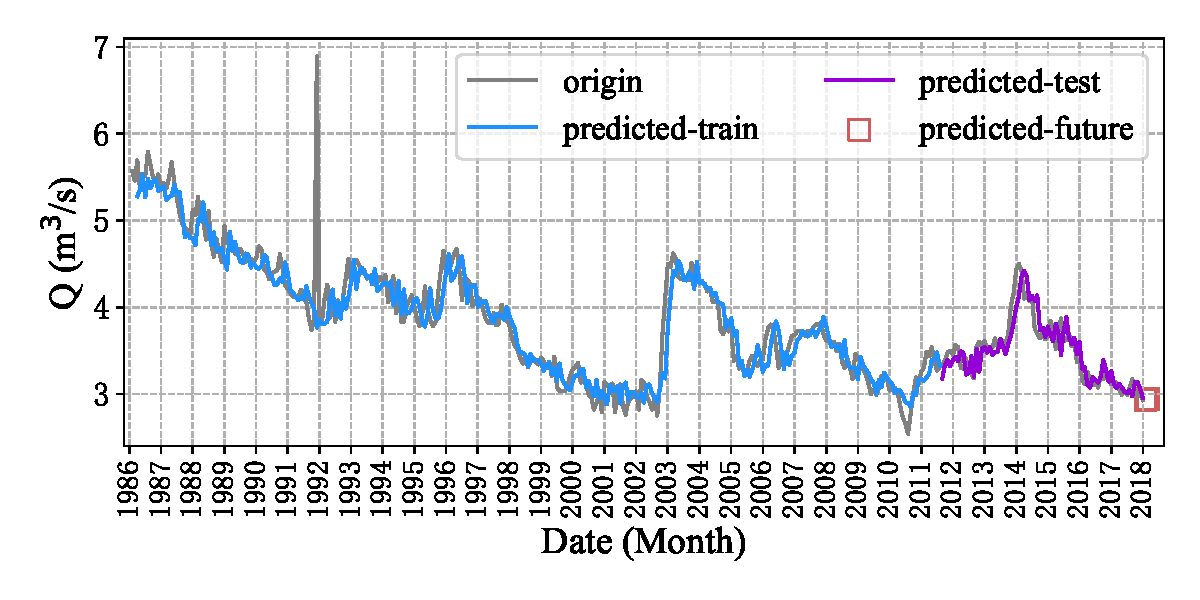
\includegraphics[width=\textwidth]{Img/chap4_spr/out2/spr_series_in_1_out_2_lstm_cnn.pdf}
    \vspace{-1.2cm}
    \caption{LSTM-1DCNN ($I_{-1}$)}
    \label{fig:spr_series_in_1_out_2_lstm_cnn}
  \end{subfigure}
  \\
  \begin{subfigure}[b]{0.305\textwidth}
    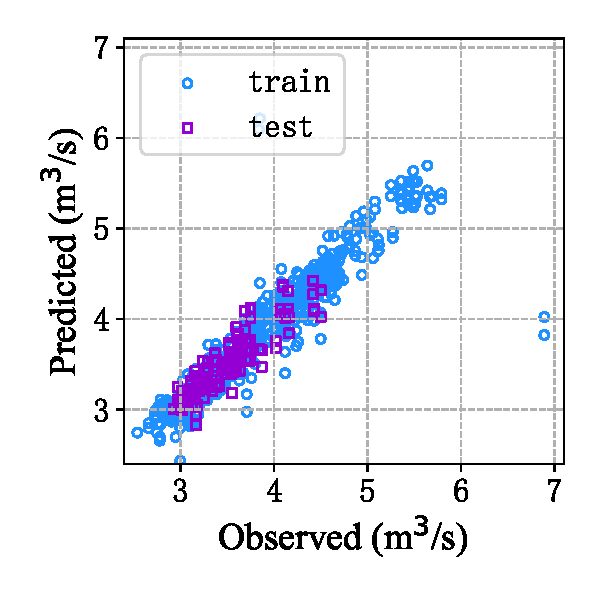
\includegraphics[width=\textwidth]{Img/chap4_spr/out2/spr_scatter_in_2_out_2_svr.pdf}
    \vspace{-1.2cm}
    \caption{SVR ($I_{-2}$)}
    \label{fig:spr_scatter_in_2_out_2_svr}
  \end{subfigure}
  ~
  \begin{subfigure}[b]{0.615\textwidth}
    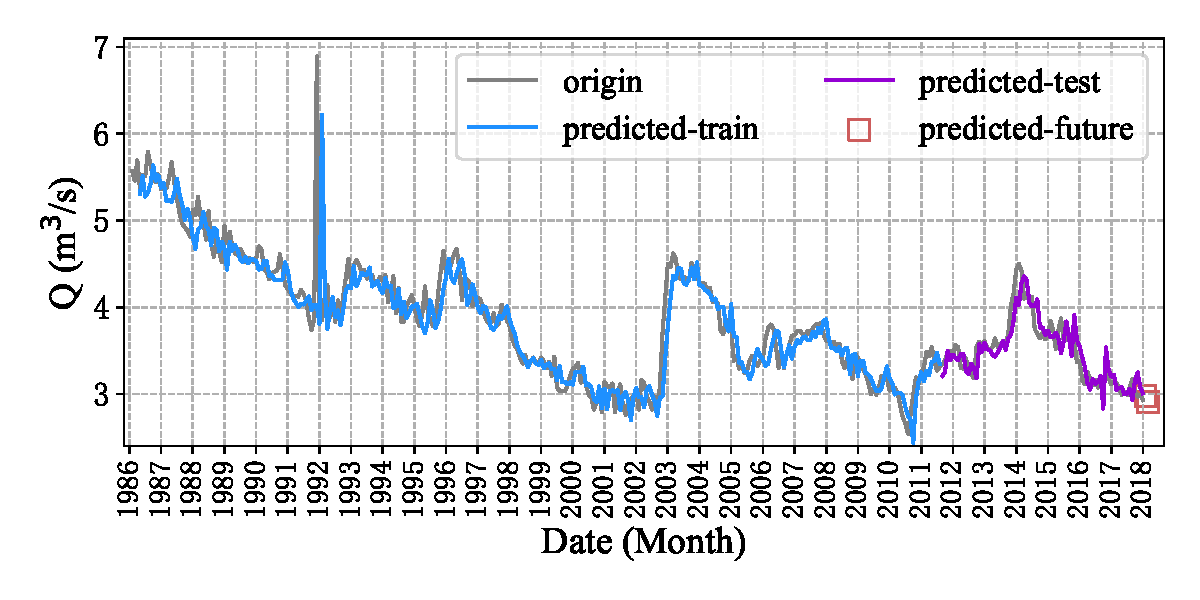
\includegraphics[width=\textwidth]{Img/chap4_spr/out2/spr_series_in_2_out_2_svr.pdf}
    \vspace{-1.2cm}
    \caption{SVR ($I_{-2}$)}
    \label{fig:spr_series_in_2_out_2_svr}
  \end{subfigure}
  \\
  \centering
  \begin{subfigure}[b]{0.305\textwidth}
    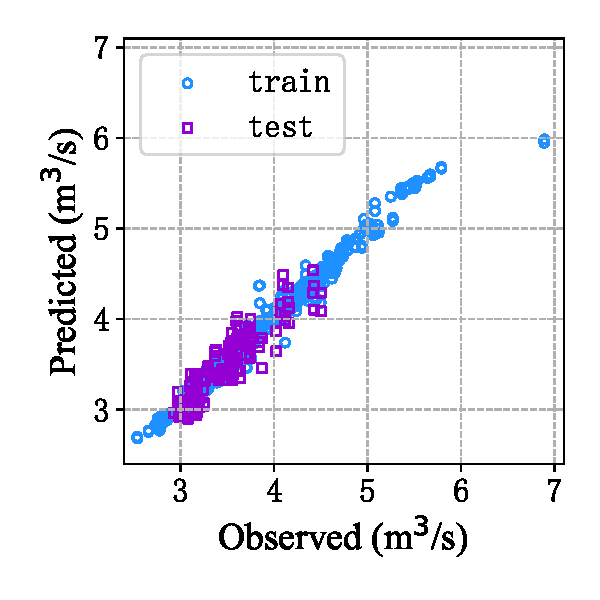
\includegraphics[width=\textwidth]{Img/chap4_spr/out2/spr_scatter_in_3_out_2_rf.pdf}
    \vspace{-1.2cm}
    \caption{RF ($I_{-3}$)}
    \label{fig:spr_scatter_in_3_out_2_rf}
  \end{subfigure}
  ~
  \begin{subfigure}[b]{0.615\textwidth}
    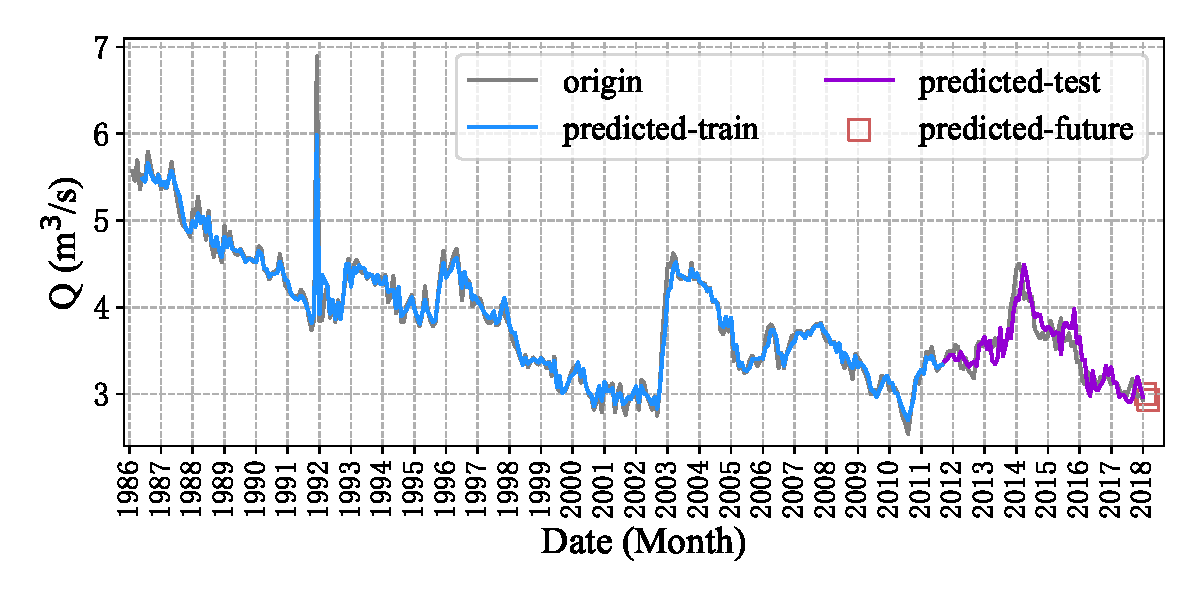
\includegraphics[width=\textwidth]{Img/chap4_spr/out2/spr_series_in_3_out_2_rf.pdf}
    \vspace{-1.2cm}
    \caption{RF ($I_{-3}$)}
    \label{fig:spr_series_in_3_out_2_rf}
  \end{subfigure}
  \\
  \begin{subfigure}[b]{0.305\textwidth}
    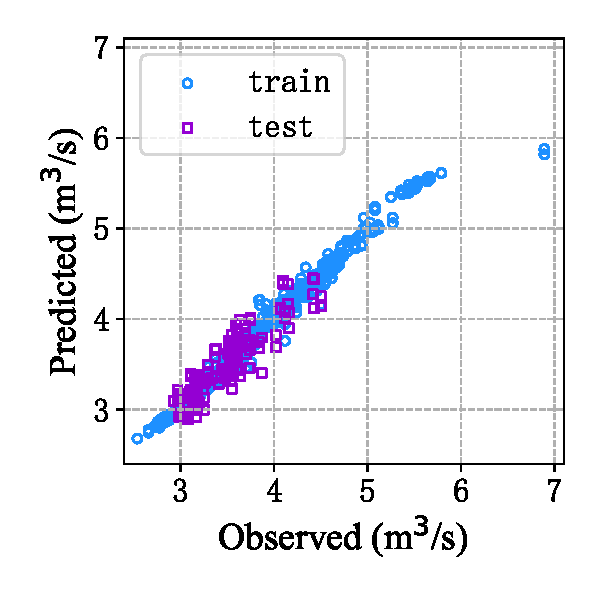
\includegraphics[width=\textwidth]{Img/chap4_spr/out2/spr_scatter_in_4_out_2_rf.pdf}
    \vspace{-1.2cm}
    \caption{RF ($I_{-4}$)}
    \label{fig:spr_scatter_in_4_out_2_rf}
  \end{subfigure}
  ~
  \begin{subfigure}[b]{0.615\textwidth}
    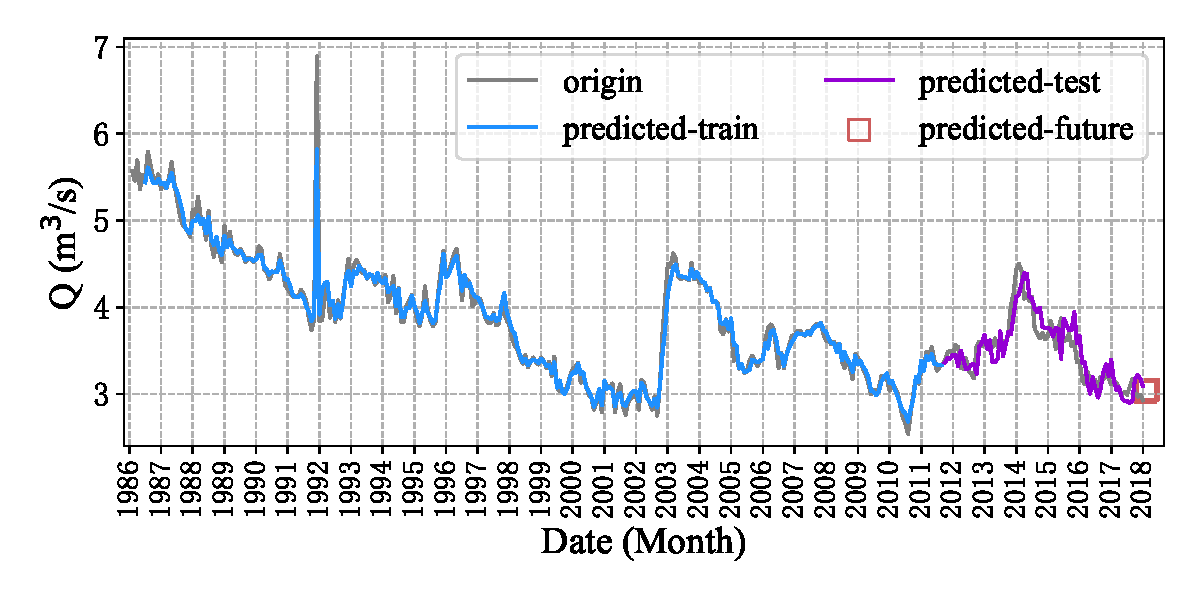
\includegraphics[width=\textwidth]{Img/chap4_spr/out2/spr_series_in_4_out_2_rf.pdf}
    \vspace{-1.2cm}
    \caption{RF ($I_{-4}$)}
    \label{fig:spr_series_in_4_out_2_rf}
  \end{subfigure}
  \bicaption[不同输入时间窗口下最佳模型预测未来2个月的泉流量]{不同输入时间窗口下最佳模型预测未来2个月的泉流量。}{Predicting the next two monthly spring discharge by the best models with different input windows.}
  \label{fig:spr_out_2}
\end{figure}

图\ref{fig:spr_out_2}绘制了不同输入时间窗口下最佳模型预测未来2个月的泉流量$O_{+2}$,只展示了每个输入样本的最后一个预测值。由图\ref{fig:spr_out_2}可知,对于预测值和测试集,RF具备良好的拟合能力,且训练集中预测值和观测值时间上不存在偏差,测试集中预测值和观测值时间上存在2个月的偏差;LSTM-1DCNN和SVR所有的预测值和观测值在时间上存在2个月的偏差。绝大多数的预测值和观测值的绝对误差基本在$\SI{0.2}{m^{3}/s}$以内。利用最佳的RF预测未来2个月(即2019年1月和2月)龙子祠泉流量,均可得到较为理想的结果。

\subsection{预测未来3个月的泉流量}\label{sec:spr_three}

\begin{table}[!htbp]
  \centering
  \bicaption[最佳模型预测2019年1月至3月的泉流量]{最佳模型预测2019年至3月的泉流量。}{Prediction the spring discharge from March 2019 to February 2019.}
  \label{tab:spr_three}
  \footnotesize
  \begin{tabular}{ccccc}
    \toprule
    输入时间窗口 & 1 & 2 & 3 & 4 \\
    \midrule
    2019年1月的泉流量($\SI{}{m^{3}/s}$)& \textbf{2.98} & 2.98 & 3.03 & 3.06  \\
    2019年2月的泉流量($\SI{}{m^{3}/s}$)& \textbf{2.98} & 2.91 & 3.04 & 3.07  \\
    2019年3月的泉流量($\SI{}{m^{3}/s}$)& \textbf{2.89} & 2.90 & 2.98 & 2.99  \\
    \bottomrule
  \end{tabular}
\end{table}

本节讨论输出时间窗口为3个月的情况。表\ref{tab:spr_indicates}中第七、八列展示了测试阶段不同模型和输入时间窗口预测未来3个月泉流量的拟合指标效果。表\ref{tab:spr_three}展示了不同输入时间窗口下,利用最佳模型预测未来3个月的泉流量变化。当输入时间窗口为1个月时,LSTM-1DCNN拟合指标MSE=$\SI{0.0015}{m^{3}/s}$,RMSE=$\SI{0.0389}{m^{3}/s}$,预测2019年1月的泉流量为$\SI{2.98}{m^{3}/s}$,2019年2月的泉流量为$\SI{2.98}{m^{3}/s}$,2019年3月的泉流量为$\SI{2.89}{m^{3}/s}$;当输入时间窗口为2个月时,SVR拟合指标MSE=\\$\SI{0.0013}{m^{3}/s}$,RMSE=$\SI{0.0360}{m^{3}/s}$,预测2019年1月的泉流量为$\SI{2.98}{m^{3}/s}$,2019年2月的泉流量为$\SI{2.91}{m^{3}/s}$,2019年3月的泉流量为$\SI{2.90}{m^{3}/s}$;当输入时间窗口为3个月时,LSTM-RNN拟合指标MSE=$\SI{0.0015}{m^{3}/s}$,RMSE=$\SI{0.0390}{m^{3}/s}$,预测2019年1月的泉流量为$\SI{2.30}{m^{3}/s}$,2019年2月的泉流量为$\SI{2.94}{m^{3}/s}$,2019年3月的泉流量为$\SI{2.86}{m^{3}/s}$;当输入时间窗口为4个月时,RF拟合指标MSE=$\SI{0.0017}{m^{3}/s}$,RMSE=$\SI{0.0414}{m^{3}/s}$,预测2019年1月的泉流量为$\SI{3.06}{m^{3}/s}$,2019年2月的泉流量为$\SI{3.07}{m^{3}/s}$,2019年3月的泉流量为$\SI{2.99}{m^{3}/s}$。

\begin{figure}[!htbp]
  \centering
  \begin{subfigure}[b]{0.305\textwidth}
    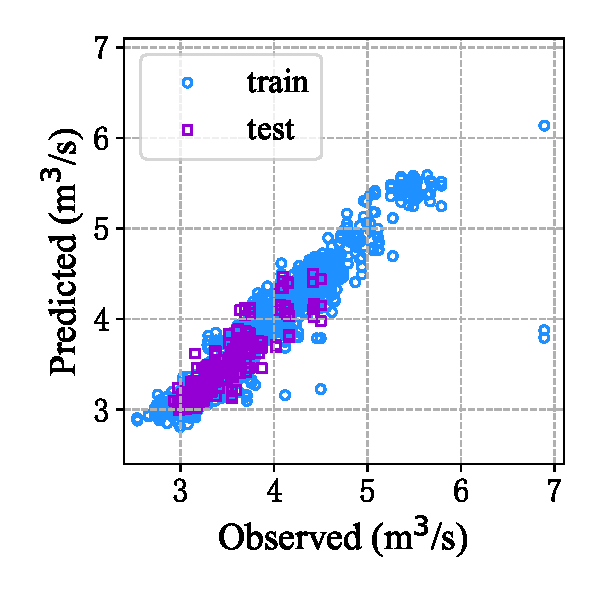
\includegraphics[width=\textwidth]{Img/chap4_spr/out3/spr_scatter_in_1_out_3_lstm_cnn.pdf}
    \vspace{-1.2cm}
    \caption{LSTM-1DCNN ($I_{-1}$)}
    \label{fig:spr_scatter_in_1_out_3_lstm_cnn}
  \end{subfigure}
  ~
  \begin{subfigure}[b]{0.615\textwidth}
    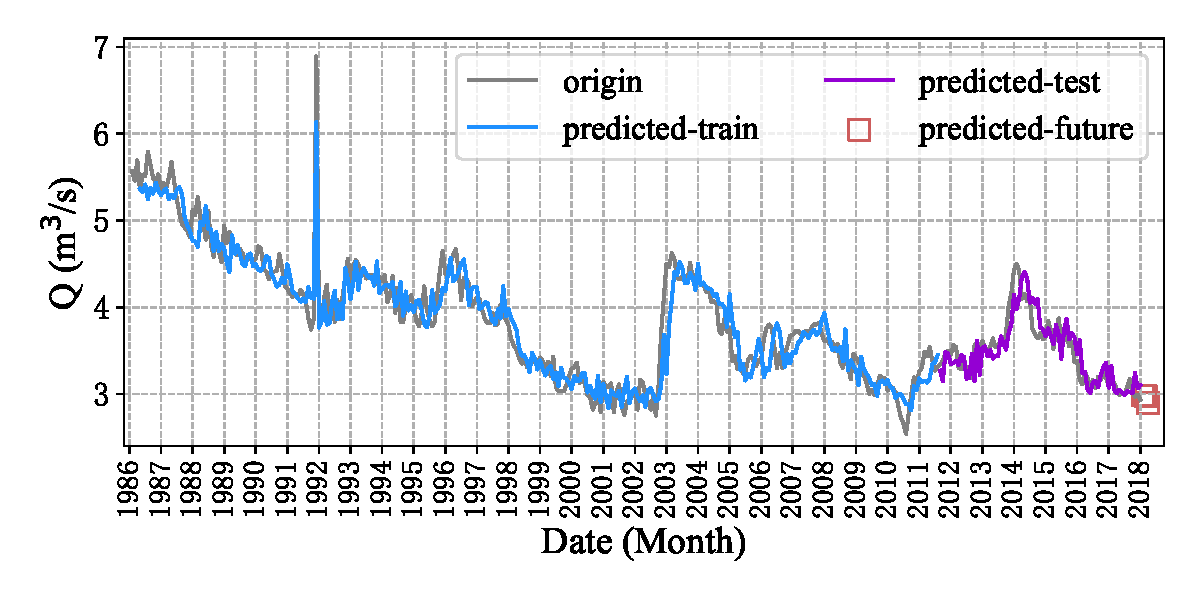
\includegraphics[width=\textwidth]{Img/chap4_spr/out3/spr_series_in_1_out_3_lstm_cnn.pdf}
    \vspace{-1.2cm}
    \caption{LSTM-1DCNN ($I_{-1}$)}
    \label{fig:spr_series_in_1_out_3_lstm_cnn}
  \end{subfigure}
  \\
  \begin{subfigure}[b]{0.305\textwidth}
    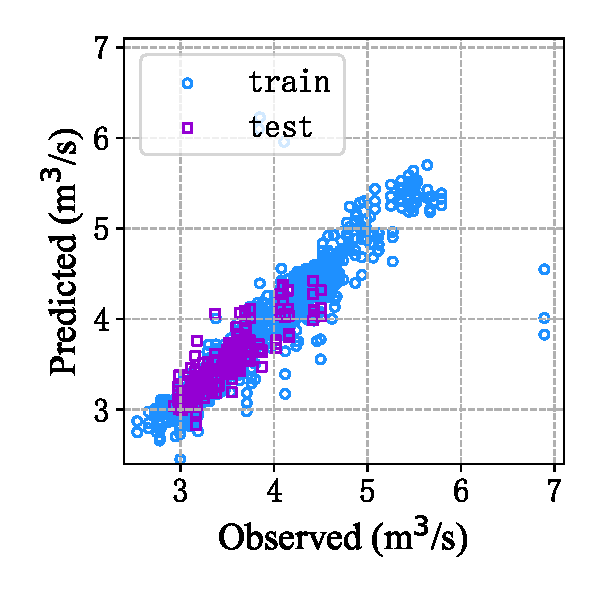
\includegraphics[width=\textwidth]{Img/chap4_spr/out3/spr_scatter_in_2_out_3_svr.pdf}
    \vspace{-1.2cm}
    \caption{SVR ($I_{-2}$)}
    \label{fig:spr_scatter_in_2_out_3_svr}
  \end{subfigure}
  ~
  \begin{subfigure}[b]{0.615\textwidth}
    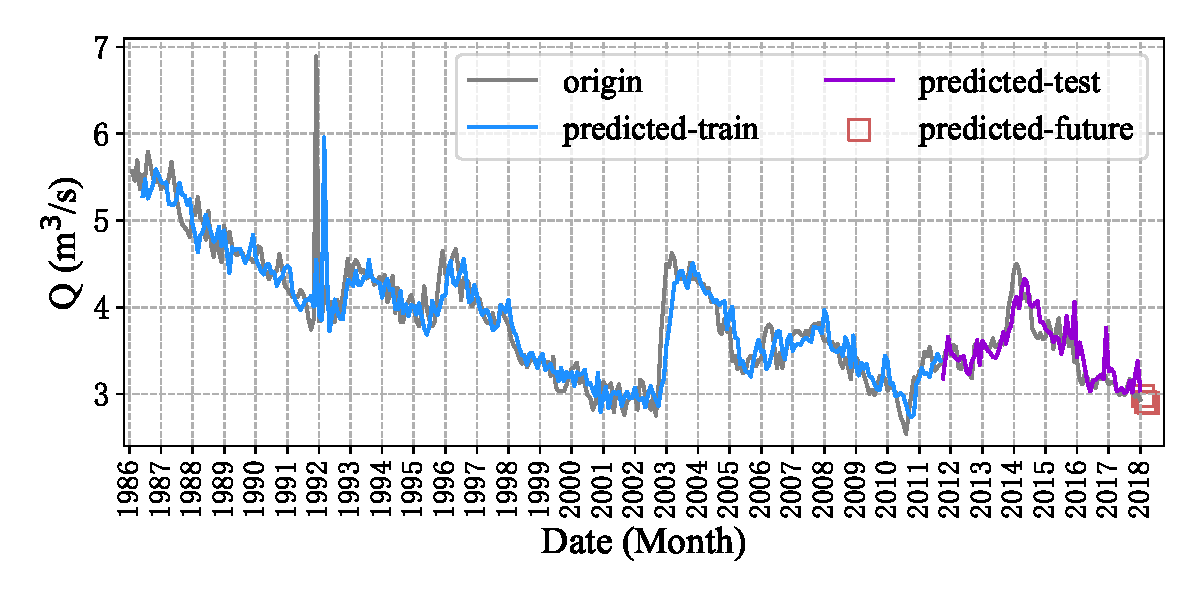
\includegraphics[width=\textwidth]{Img/chap4_spr/out3/spr_series_in_2_out_3_svr.pdf}
    \vspace{-1.2cm}
    \caption{SVR ($I_{-2}$)}
    \label{fig:spr_series_in_2_out_3_svr}
  \end{subfigure}
  \\
  \begin{subfigure}[b]{0.305\textwidth}
    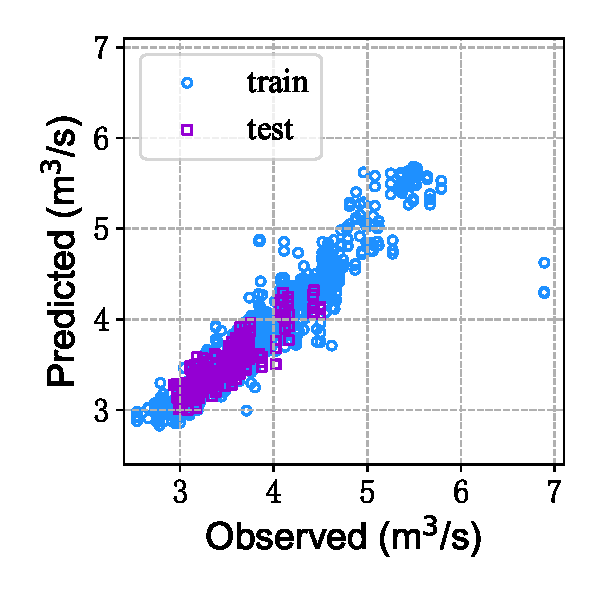
\includegraphics[width=\textwidth]{Img/chap4_spr/out3/spr_scatter_in_3_out_3_lstm.pdf}
    \vspace{-1.2cm}
    \caption{LSTM-RNN ($I_{-3}$)}
    \label{fig:spr_scatter_in_3_out_3_lstm}
  \end{subfigure}
  ~
  \begin{subfigure}[b]{0.615\textwidth}
    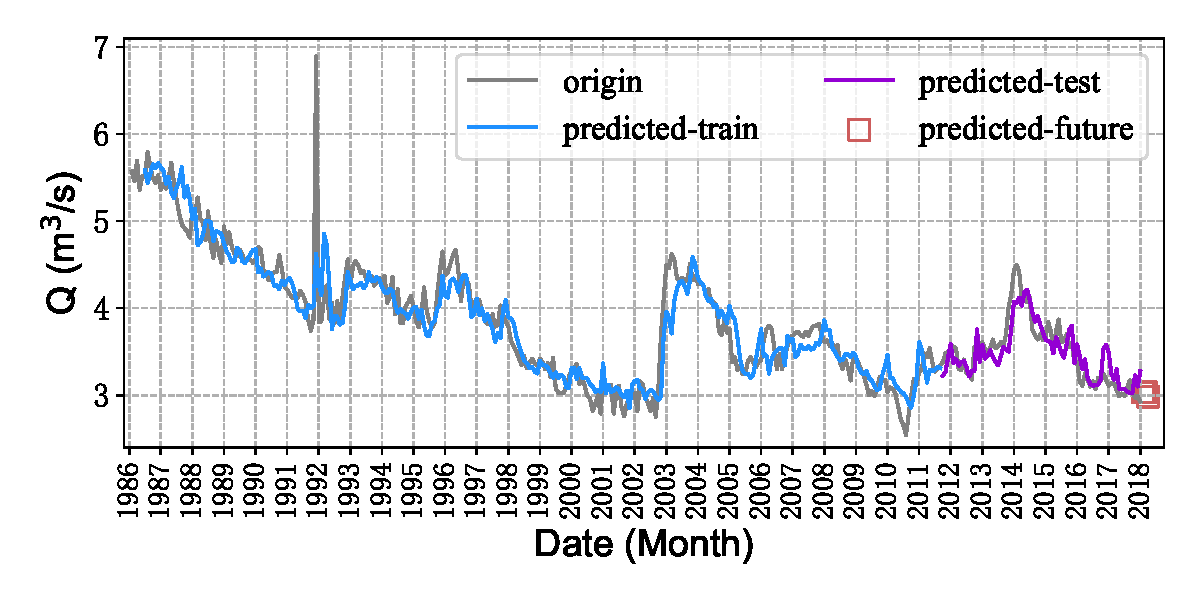
\includegraphics[width=\textwidth]{Img/chap4_spr/out3/spr_series_in_3_out_3_lstm.pdf}
    \vspace{-1.2cm}
    \caption{LSTM-RNN ($I_{-3}$)}
    \label{fig:spr_series_in_3_out_3_lstm}
  \end{subfigure}
  \\
  \begin{subfigure}[b]{0.305\textwidth}
    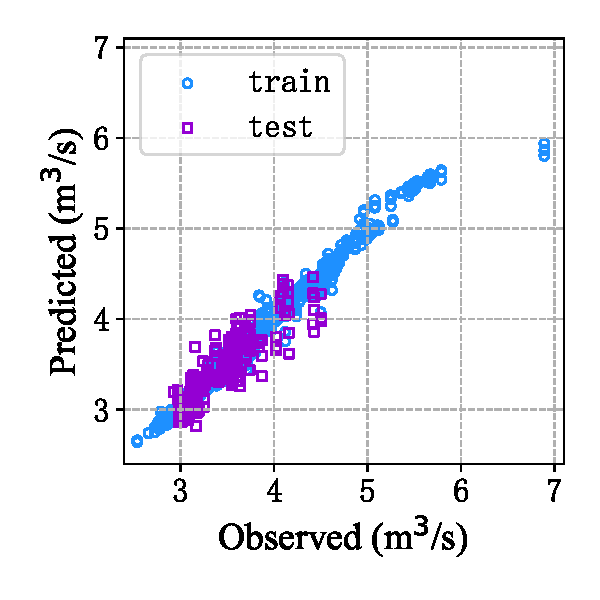
\includegraphics[width=\textwidth]{Img/chap4_spr/out3/spr_scatter_in_4_out_3_rf.pdf}
    \vspace{-1.2cm}
    \caption{RF ($I_{-4}$)}
    \label{fig:spr_scatter_in_4_out_3_rf}
  \end{subfigure}
  ~
  \begin{subfigure}[b]{0.615\textwidth}
    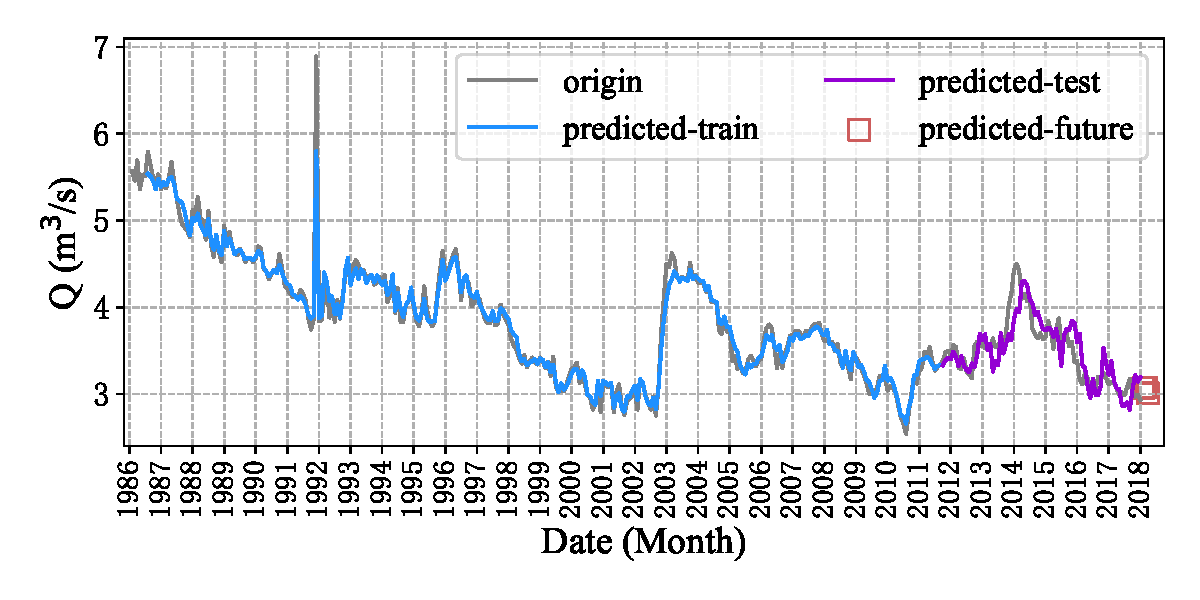
\includegraphics[width=\textwidth]{Img/chap4_spr/out3/spr_series_in_4_out_3_rf.pdf}
    \vspace{-1.2cm}
    \caption{RF ($I_{-4}$)}
    \label{fig:spr_series_in_4_out_3_rf}
  \end{subfigure}
  \bicaption[不同输入时间窗口下最佳模型预测未来3个月的泉流量]{不同输入时间窗口下最佳模型预测未来3个月的泉流量。}{Predicting the next three monthly spring discharge by the best models with different input windows.}
  \label{fig:spr_out_3}
\end{figure}

图\ref{fig:spr_out_3}绘制了不同输入时间窗口下最佳模型预测未来3个月的泉流量$O_{+3}$,只展示了每个输入样本的最后一个预测值。由图\ref{fig:spr_out_3}可知,对于预测值和测试集,RF具备良好的拟合能力,且训练集中预测值和观测值时间上不存在偏差,测试集中预测值和观测值时间上存在3个月的偏差;LSTM-1DCNN、SVR和LSTM的预测值和观测值在时间上存在3个月的偏差。绝大多数的预测值和观测值的绝对误差基本在$\SI{0.3}{m^{3}/s}$以内。利用这些最佳模型预测未来3个月(即2019年1月、2月和3月)龙子祠泉流量,均可得到较为可靠的结果。

\subsection{预测未来4个月的泉流量}\label{sec:spr_four}

\begin{table}[!htbp]
  \centering
  \bicaption[最佳模型预测2019年1月至4月的泉流量]{最佳模型预测2019年1月至4月的泉流量。}{Prediction the spring discharge in April 2019, March 2019, Junarary 2019 and Februar 2019.}
  \label{tab:spr_four}
  \footnotesize
  \begin{tabular}{ccccc}
    \toprule
    输入时间窗口 & 1 & 2 & 3 & 4\\
    \midrule
    2019年1月的泉流量($\SI{}{m^{3}/s}$)& \textbf{2.97} & 2.98 & 2.30 & 3.07 \\
    2019年2月的泉流量($\SI{}{m^{3}/s}$)& \textbf{2.91} & 2.91 & 2.91 & 3.01 \\
    2019年3月的泉流量($\SI{}{m^{3}/s}$)& \textbf{2.91} & 2.90 & 2.83 & 2.97 \\
    2019年4月的泉流量($\SI{}{m^{3}/s}$)& \textbf{2.90} & 2.93 & 2.78 & 2.93 \\
    \bottomrule
  \end{tabular}
\end{table}

本节讨论输出时间窗口为4个月的情况。表\ref{tab:spr_indicates}中第九、十列展示了测试阶段使用不同模型和输入时间窗口预测未来4个月泉流量的拟合指标效果。表\ref{tab:spr_four}展示了不同输入时间窗口下,利用最佳模型预测未来4个月的泉流量变化趋势。从表\ref{tab:spr_four}可知,2019年1月至2019年4月泉流量略微有所下降。

当输入时间窗口为1个月时,SVR拟合指标MSE=$\SI{0.0019}{m^{3}/s}$,RMSE=\\$\SI{0.0433}{m^{3}/s}$,预测2019年1月的泉流量为$\SI{2.97}{m^{3}/s}$,2019年2月的泉流量为$\SI{2.91}{m^{3}/s}$,2019年3月的泉流量为$\SI{2.91}{m^{3}/s}$,2019年4月的泉流量为$\SI{2.90}{m^{3}/s}$;当输入时间窗口为2个月时,SVR拟合指标MSE=$\SI{0.0018}{m^{3}/s}$,RMSE=$\SI{0.0424}{m^{3}/s}$,预测2019年1月的泉流量为$\SI{2.98}{m^{3}/s}$,2019年2月的泉流量为$\SI{2.91}{m^{3}/s}$,2019年3月的泉流量为$\SI{2.90}{m^{3}/s}$,2019年4月的泉流量为$\SI{2.93}{m^{3}/s}$;当输入时间窗口为3个月时,SVR拟合指标MSE=$\SI{0.0020}{m^{3}/s}$,RMSE=$\SI{0.0448}{m^{3}/s}$,预测2019年1月的泉流量为$\SI{2.30}{m^{3}/s}$,2019年2月的泉流量为$\SI{2.91}{m^{3}/s}$,2019年3月的泉流量为$\SI{2.83}{m^{3}/s}$,2019年4月的泉流量为$\SI{2.77}{m^{3}/s}$;当输入时间窗口为4个月时,RF拟合指标MSE=$\SI{0.0022}{m^{3}/s}$,RMSE=$\SI{0.0468}{m^{3}/s}$,预测2019年1月的泉流量为$\SI{3.07}{m^{3}/s}$,2019年2月的泉流量为$\SI{3.01}{m^{3}/s}$,2019年3月的泉流量为$\SI{2.97}{m^{3}/s}$,2019年4月的泉流量为$\SI{2.93}{m^{3}/s}$。

\begin{figure}[!htbp]
  \centering
  \begin{subfigure}[b]{0.305\textwidth}
    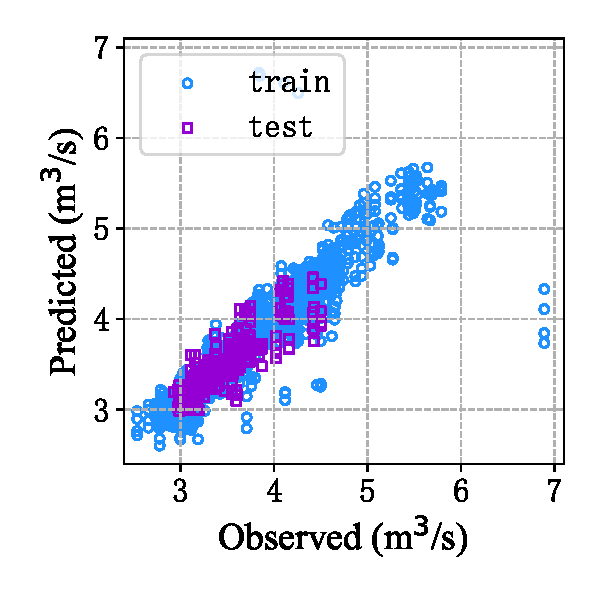
\includegraphics[width=\textwidth]{Img/chap4_spr/out4/spr_scatter_in_1_out_4_svr.pdf}
    \vspace{-1.2cm}
    \caption{SVR ($I_{-1}$)}
    \label{fig:spr_scatter_in_1_out_4_svr}
  \end{subfigure}
  ~
  \begin{subfigure}[b]{0.615\textwidth}
    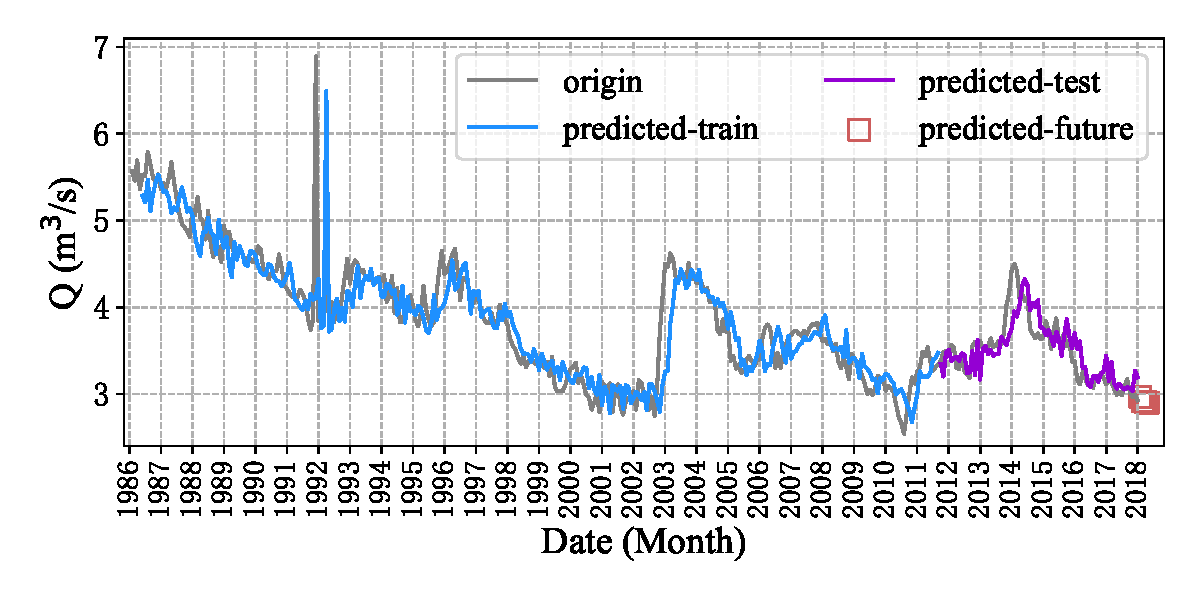
\includegraphics[width=\textwidth]{Img/chap4_spr/out4/spr_series_in_1_out_4_svr.pdf}
    \vspace{-1.2cm}
    \caption{SVR ($I_{-1}$)}
    \label{fig:spr_series_in_1_out_4_svr}
  \end{subfigure}
  \\
  \begin{subfigure}[b]{0.305\textwidth}
    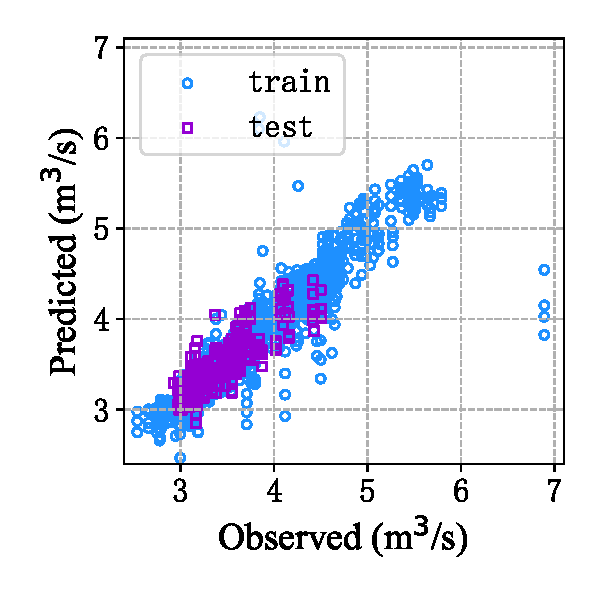
\includegraphics[width=\textwidth]{Img/chap4_spr/out4/spr_scatter_in_2_out_4_svr.pdf}
    \vspace{-1.2cm}
    \caption{SVR ($I_{-2}$)}
    \label{fig:spr_scatter_in_2_out_4_svr}
  \end{subfigure}
  ~
  \begin{subfigure}[b]{0.615\textwidth}
    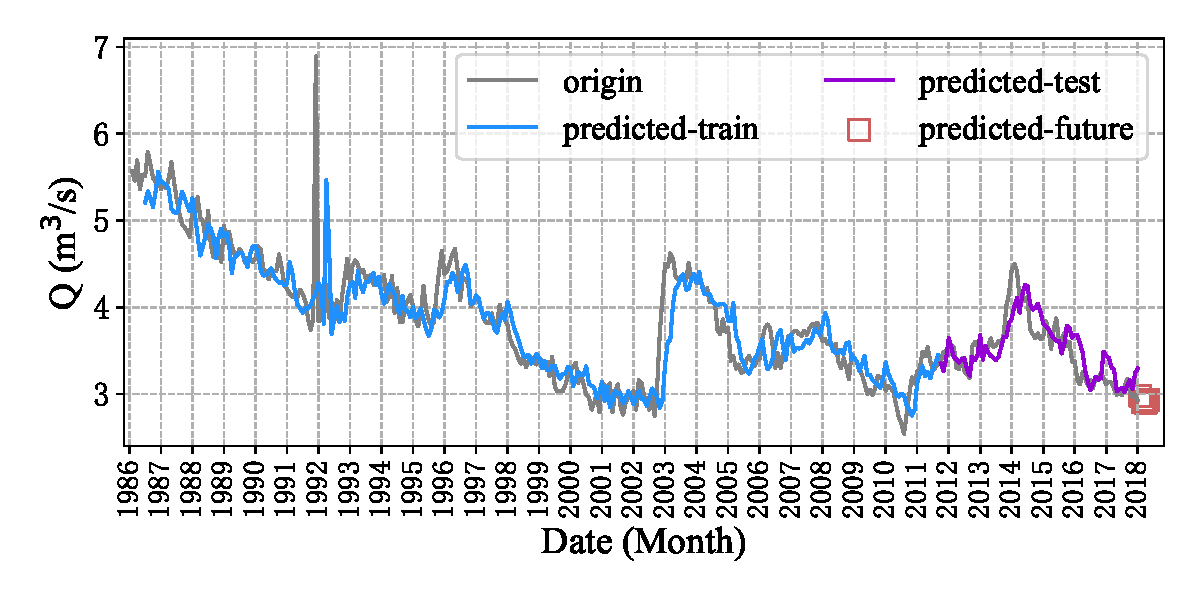
\includegraphics[width=\textwidth]{Img/chap4_spr/out4/spr_series_in_2_out_4_svr.pdf}
    \vspace{-1.2cm}
    \caption{SVR ($I_{-2}$)}
    \label{fig:spr_series_in_2_out_4_svr}
  \end{subfigure}
  \\
  \begin{subfigure}[b]{0.305\textwidth}
    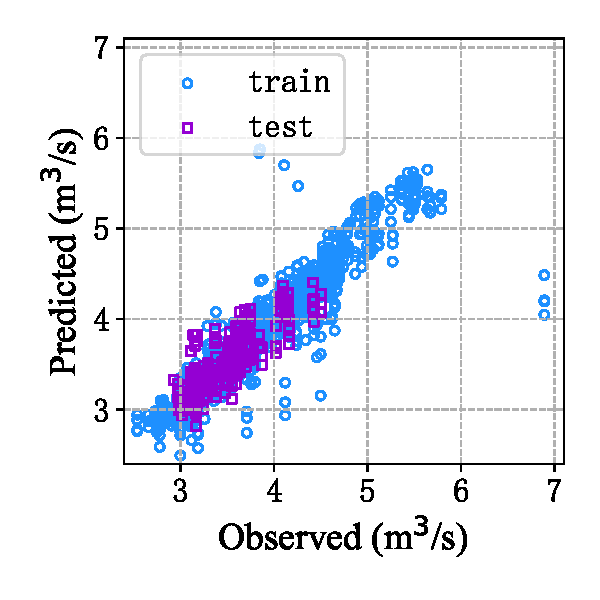
\includegraphics[width=\textwidth]{Img/chap4_spr/out4/spr_scatter_in_3_out_4_svr.pdf}
    \vspace{-1.2cm}
    \caption{SVR ($I_{-3}$)}
    \label{fig:spr_scatter_in_3_out_4_svr}
  \end{subfigure}
  ~
  \begin{subfigure}[b]{0.615\textwidth}
    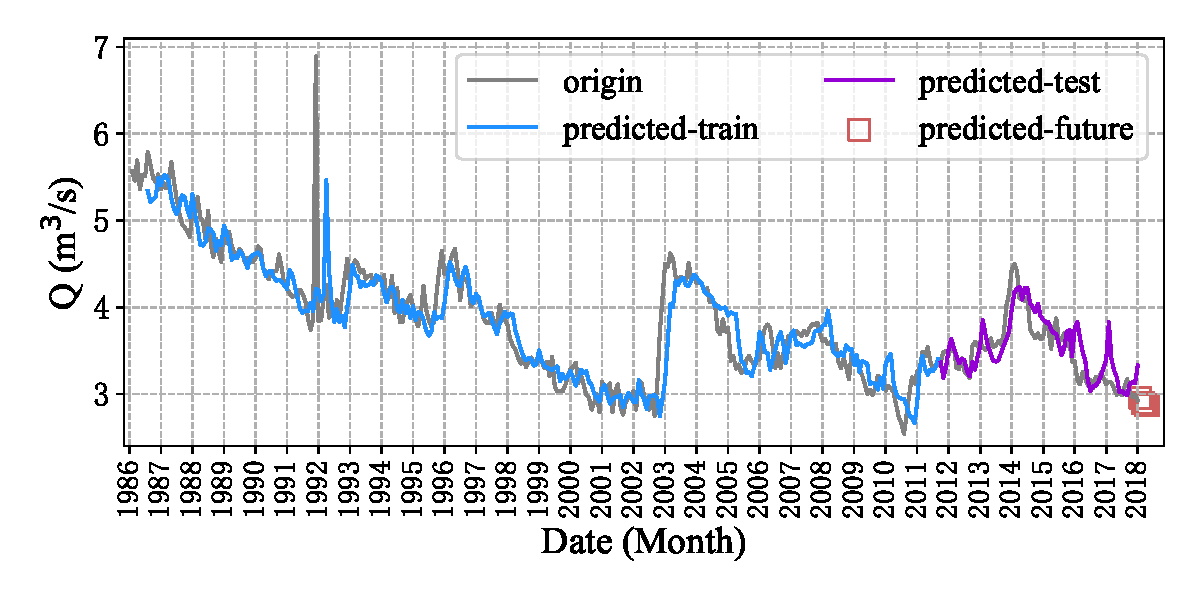
\includegraphics[width=\textwidth]{Img/chap4_spr/out4/spr_series_in_3_out_4_svr.pdf}
    \vspace{-1.2cm}
    \caption{SVR ($I_{-3}$)}
    \label{fig:spr_series_in_3_out_4_svr}
  \end{subfigure}
  \\
  \begin{subfigure}[b]{0.305\textwidth}
    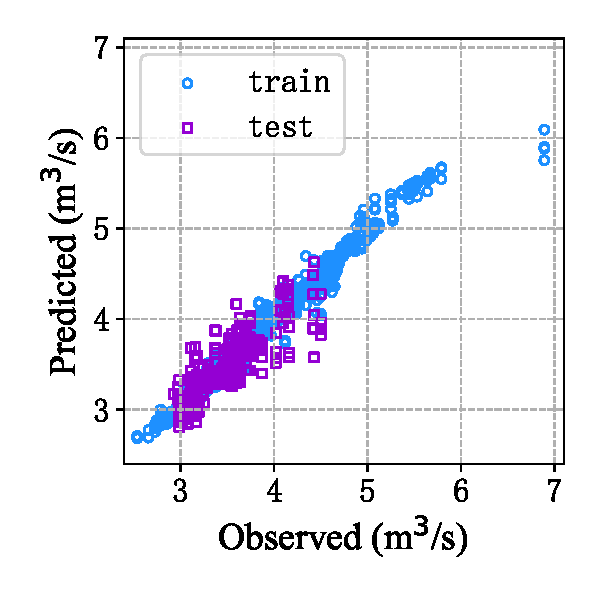
\includegraphics[width=\textwidth]{Img/chap4_spr/out4/spr_scatter_in_4_out_4_rf.pdf}
    \vspace{-1.2cm}
    \caption{RF ($I_{-4}$)}
    \label{fig:spr_scatter_in_4_out_4_rf}
  \end{subfigure}
  ~
  \begin{subfigure}[b]{0.615\textwidth}
    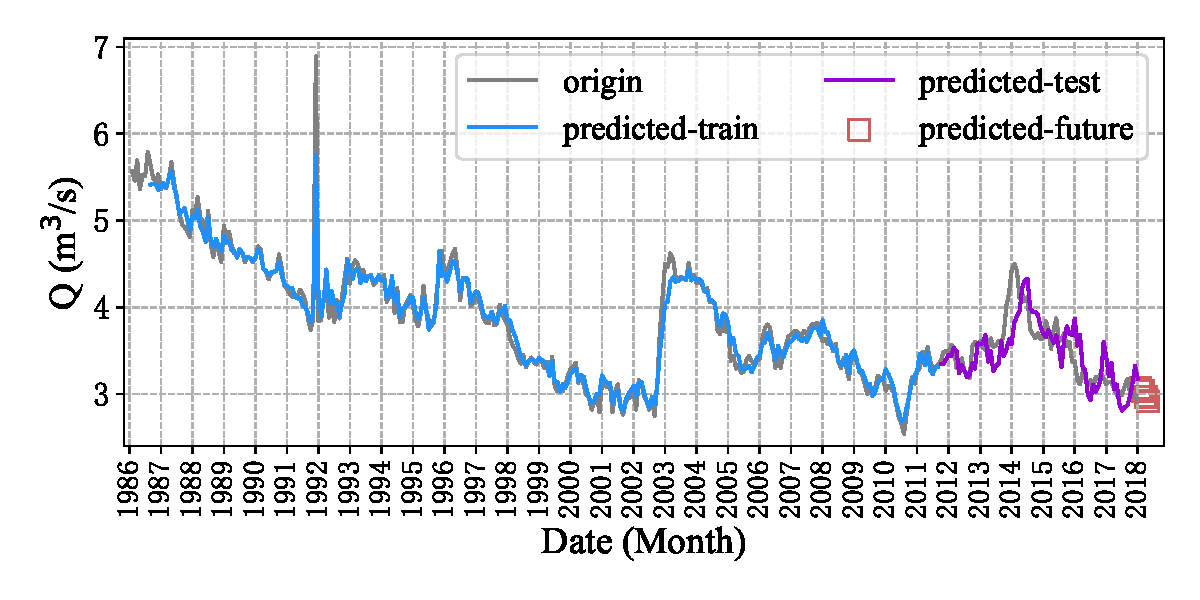
\includegraphics[width=\textwidth]{Img/chap4_spr/out4/spr_series_in_4_out_4_rf.pdf}
    \vspace{-1.2cm}
    \caption{RF ($I_{-4}$)}
    \label{fig:spr_series_in_4_out_4_rf}
  \end{subfigure}
  \bicaption[不同输入时间窗口下最佳模型预测未来4个月的泉流量]{不同输入时间窗口下最佳模型预测未来4个月的泉流量。}{Predicting the next four monthly spring discharge by the best models with different input windows.}
  \label{fig:spr_out_4}
\end{figure}

图\ref{fig:spr_out_4}绘制了不同输入时间窗口下最佳模型预测未来4个月的泉流量$O_{+4}$,只展示了每个输入样本的最后一个预测值。由图\ref{fig:spr_out_4}可知,对于预测值和测试集,RF具备良好的拟合能力,且训练集中预测值和观测值时间上不存在偏差,测试集中预测值和观测值时间上存在4个月的偏差;SVR中所有的预测值和观测值都存在4个月的偏差。绝大多数的预测值和观测值的绝对误差基本在$\SI{0.5}{m^{3}/s}$以内。利用这些最佳模型预测未来4个月(即2019年1月、2月、3月和4月)龙子祠泉流量,得到泉流量具有一定的可靠性。

\subsection{利用历史泉流量预测未来泉流量}\label{sec:spr_only}

本节考虑输入中仅有泉流量时预测未来泉流量走势情况。当输入和输出时间窗口均为1个月时,未来1个月的泉流量为$Q(t+1)=f(Q(t))$。具备一维卷积的神经网络其输入需要具备高维特征,因此本节只使用LSTM-RNN。经过不断测试,发现3层的LSTM-RNN最优,且两个隐藏层的LSTM单元数分别为64和32。表\ref{tab:spr_indicators_only_out_1}展示了基于不同模型利用历史1个月的泉流量预测未来1个月的泉流量的拟合指标效果,其中LSTM-RNN和SVR的性能最佳。表\ref{tab:spr_pre_only_out_1}展示了不同模型利用历史1个月的泉流量预测2019年1月的泉流量。

\begin{table}[!htbp]
  \centering
  \bicaption[不同模型利用历史1个月的泉流量预测未来1个月的泉流量的拟合指标效果]{不同模型利用历史1个月的泉流量预测未来1个月的泉流量的拟合指标效果。}{The indicators for predicting the next monthly spring discharge by different models with one input window.}
  \label{tab:spr_indicators_only_out_1}
  \footnotesize
  \renewcommand{\arraystretch}{1}
  \begin{tabular}{ccccc}
    \toprule
    \multirow{2}{*}{模型} & \multicolumn{2}{c}{训练集} & \multicolumn{2}{c}{测试集}\\
    \cmidrule(lr){2-3} \cmidrule(lr){4-5}
    \noalign{\smallskip}
    & MSE & RMSE & MSE & RMSE \\
    \midrule 
    LSTM-RNN & 0.0029 & 0.0540 & \textbf{0.0009} & \textbf{0.0297} \\
    SVR & 0.0043 & 0.0659 & \textbf{0.0009} & \textbf{0.0297} \\
    LR & 0.0043 & 0.0655 & 0.0009 & 0.0306 \\
    RF & 0.0018 & 0.0421 & 0.0014 & 0.0374 \\
    DT & 0.0016 & 0.0400 & 0.0017 & 0.0409 \\
    KNN & 0.0026 & 0.0506 & 0.0015 & 0.0388 \\
    \bottomrule
  \end{tabular}
\end{table}

\begin{table}[!htbp]
  \centering
  \bicaption[不同模型利用历史1个月的泉流量预测2019年1月的泉流量]{不同模型利用历史1个月的泉流量预测2019年1月的泉流量。}{Predicting the monthly spring discharge  in April 2019 by different models with one input window.}
  \label{tab:spr_pre_only_out_1}
  \footnotesize
  \renewcommand{\arraystretch}{1}
  \begin{tabular}{ccccccc}
    \toprule
    模型 & LSTM-RNN & SVR & LR & RF & DT & KNN\\
    \midrule 
    2019年1月的泉流量($\SI{}{m^{3}/s}$) & 2.98 & 2.97 & 3.01 & 2.94 & 2.97 & 2.91 \\
    \bottomrule
  \end{tabular}
\end{table}

当输入时间窗口为1个月时,且输入中仅含有历史泉流量,而不含泉域的降雨量时。LSTM-RNN的测试集拟合指标MSE=$\SI{0.0009}{m^{3}/s}$,RMSE=$\SI{0.0297}{m^{3}/s}$,预测2019年1月的泉流量为$\SI{2.98}{m^{3}/s}$;SVR的测试集拟合指标MSE=$\SI{0.0009}{m^{3}/s}$,RMSE=$\SI{0.0297}{m^{3}/s}$,预测2019年1月的泉流量为$\SI{2.97}{m^{3}/s}$;LR的测试集拟合指标MSE=$\SI{0.0009}{m^{3}/s}$,RMSE=$\SI{0.0306}{m^{3}/s}$,预测2019年1月的泉流量为$\SI{3.01}{m^{3}/s}$;RF的测试集拟合指标MSE=$\SI{0.0014}{m^{3}/s}$,RMSE=$\SI{0.0374}{m^{3}/s}$,预测2019年1月的泉流量为$\SI{2.94}{m^{3}/s}$;DT的测试集拟合指标MSE=$\SI{0.0017}{m^{3}/s}$,RMSE=$\SI{0.0409}{m^{3}/s}$,预测2019年1月的泉流量为$\SI{2.97}{m^{3}/s}$;KNN的测试集拟合指标MSE=$\SI{0.0015}{m^{3}/s}$,RMSE=$\SI{0.0388}{m^{3}/s}$,预测2019年1月的泉流量为$\SI{2.91}{m^{3}/s}$。

\begin{figure}[!htbp]
  \centering
  \begin{subfigure}[b]{0.305\textwidth}
    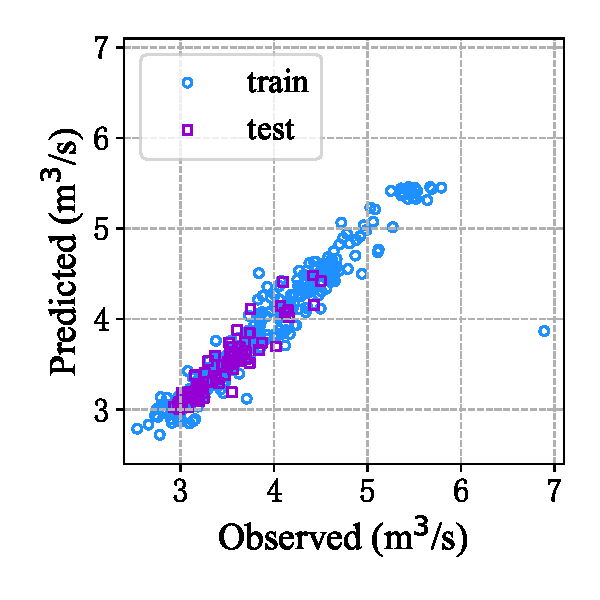
\includegraphics[width=\textwidth]{Img/chap4_spr/in_only/spr_scatter_in_1_out_1_lstm_only.pdf}
    \vspace{-1.2cm}
    \caption{LSTM-RNN ($I_{-1}$)}
    \label{fig:spr_scatter_in_1_out_1_lstm_only}
  \end{subfigure}
  ~
  \begin{subfigure}[b]{0.615\textwidth}
    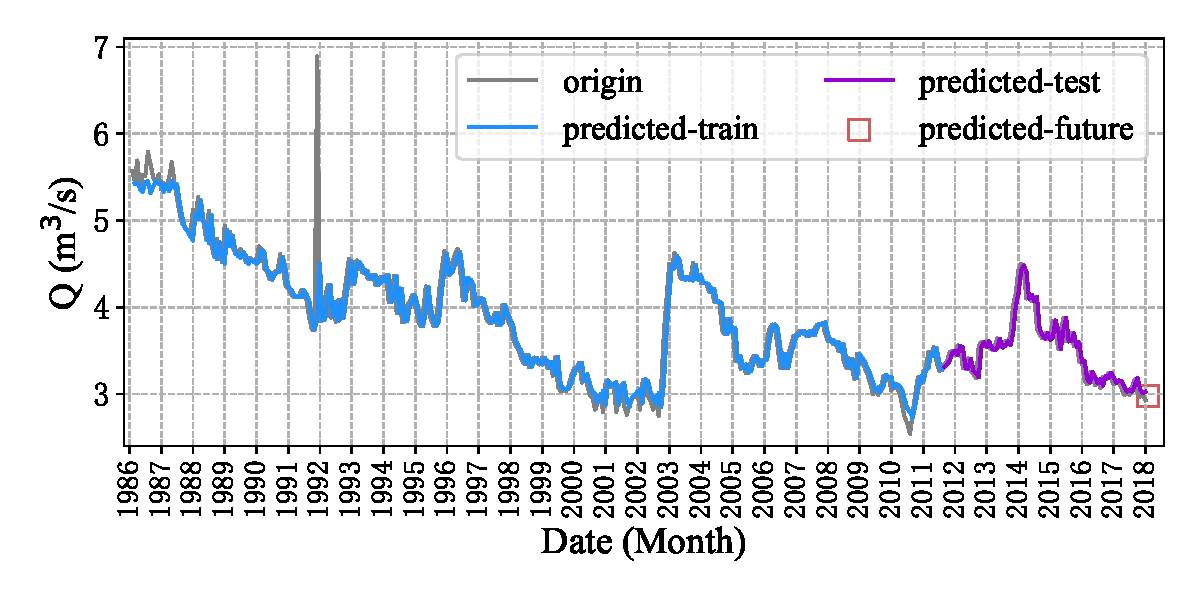
\includegraphics[width=\textwidth]{Img/chap4_spr/in_only/spr_series_in_1_out_1_lstm_only.pdf}
    \vspace{-1.2cm}
    \caption{LSTM-RNN ($I_{-1}$)}
    \label{fig:spr_series_in_1_out_1_lstm_only}
  \end{subfigure}
  \\
  \begin{subfigure}[b]{0.305\textwidth}
    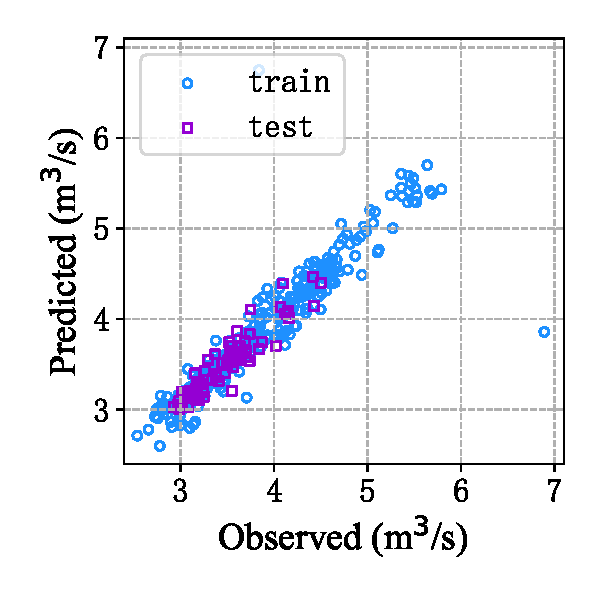
\includegraphics[width=\textwidth]{Img/chap4_spr/in_only/spr_scatter_in_1_out_1_svr_only.pdf}
    \vspace{-1.2cm}
    \caption{SVR ($I_{-1}$)}
    \label{fig:spr_scatter_in_1_out_1_svr_only}
  \end{subfigure}
  ~
  \begin{subfigure}[b]{0.615\textwidth}
    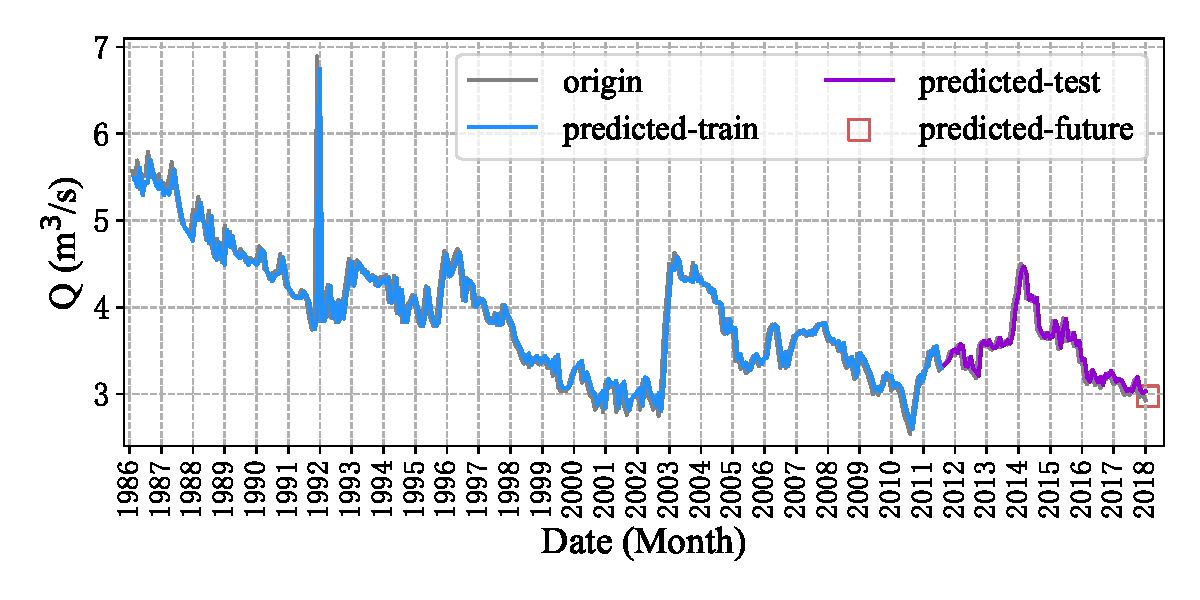
\includegraphics[width=\textwidth]{Img/chap4_spr/in_only/spr_series_in_1_out_1_svr_only.pdf}
    \vspace{-1.2cm}
    \caption{SVR ($I_{-1}$)}
    \label{fig:spr_series_in_1_out_1_svr_only}
  \end{subfigure}
  \\
  \bicaption[不同模型利用历史1个月的泉流量预测未来1个月的泉流量]{不同模型利用历史1个月的泉流量预测未来1个月的泉流量。}{Predicting the next monthly spring discharge by the different models with one input window.}
  \label{fig:spr_in_1_out_1_only}
\end{figure}


图\ref{fig:spr_in_1_out_1_only}绘制了不同模型利用历史1个月的泉流量预测未来1个月的泉流量。与图\ref{fig:spr_out_1}对比,图\ref{fig:spr_in_1_out_1_only}中LSTM-RNN和SVR也能够很好地拟合训练集和测试集,但训练集中预测值和观测值时间上存在1个月的偏差。因此,仅仅利用1个月的泉流量就能精确预测未来1个月龙子祠的泉流量。输入中只需要利用泉流量而不需要降水量信息就能够较为精确地估计未来泉流量走势,可能是降水量随季节变化,而模型学到了泉流量按季节变化的特征。

\section{讨论与小结}\label{sec:spr_conclusion}

捕获泉流量动态变化对于管理和规划水资源至关重要。许多情况下,根据历史观测的资料预测未来泉流量非常复杂。机器学习模型擅长于处理这类模型。本章使用了八种不同的机器学习算法,分别LSTM-RNN、1DCNN、LSTM-1DCNN、SVR、LR、RF、DT、KNN。选择中国山西省具备喀斯特地貌特征的龙子祠泉作为研究案例。结果显示,在可用的时间序列数据集非常有限的情况下,以上所有模型都能为预测提供较为满意的结果。从表\ref{tab:spr_indicates}得出以下结论:
\begin{enumerate}
  \item[(1)] 机器学习模型适用于捕获泉流量的动态变化过程。
  \item[(2)] 随着输入时间窗口的增加,模型性能不会大幅度提升。该结论与第\ref{sec:ss_result}章研究太阳黑子强度基本类似相同,即选择合适的输入时间窗口很关键。本研究表明输入时间窗口为1时,输入数据中含有足够的信息捕捉泉流量的动态变化。若输入时间窗口大于某个最佳值,输入数据中会产生冗余信息,这些信息在模型学习过程中会被自动忽视。极端情况下,冗余信息会导致模型产生更多的参数,使得模型更难训练,有可能会产生更大的误差。
  \item[(3)] 随着输出时间窗口的增加,模型的性能会出现一定幅度的下降。也就是说,预测未来1个月的泉流量最可靠。预测时间跨度越长,模型的性能略微有所下降。说明短期泉流量更多地由历史泉流量和降水量控制,而长期泉流量可能会更多地受到外界其他因素的干扰。在第\ref{sec:spr_background}节提到,泉流量不仅受到历史降水量和泉流量的影响,还会受到其他因素的干扰,比如地下水开采量、入渗、地表径流、蒸散、地下水补给、土壤水分、侧向水流至蓄水层、地表含水层和地下含水层之间的渗漏以及蓄水层中蓄水量的变化等。这些因素均没有被考虑到模型中。
  \item[(4)] 输入中仅考虑历史泉流量也能精确预测出未来泉流量。
  \item[(5)] 输出时间窗口大小在很大程度上决定了预测值(相对于观测值)的滞后时间。
\end{enumerate}

根据以上的研究结果,未来机器学习应用于泉流量可能的研究方向如下:
\begin{enumerate}
  \item[(1)] 本章研究对象为龙子祠泉,具有喀斯特地貌特征。可以尝试其他研究区域,进一步验证模型是否具备普适性。
  \item[(2)] 本章时间采样间隔为1个月,如果减小采样间隔时间,能否进一步提高模型的性能。
  \item[(3)] 本章尝试了8种不同的机器学习模型,并未涵盖所有机器学习模型,可以尝试其它机器学习模型或者组合这些模型,查看拟合效果能否得到进一步提升。
\end{enumerate}



